\chapter{Improving Particle Identification} \label{chap:improving_pid}

As already indicated in Section~\ref{sec:event_topologies}, particle identification (PID) is needed to perform an oscillation analysis, and improving the PID leads to increased precision when determining oscillation parameters.
The fundamental difficulty is that tracks at low energies are very hard to distinguish from cascades because the muon produced in a $\nu_\mu$-CC interaction can have low energy and will therefore not produce a long visible track.
This causes the detector response for the two event types to look very similar which can be seen in Figure~\ref{fig:topologies_low_energy}.

\begin{figure}[h]
    \centering
    \subfloat[$\nu_\mu$-CC]{
        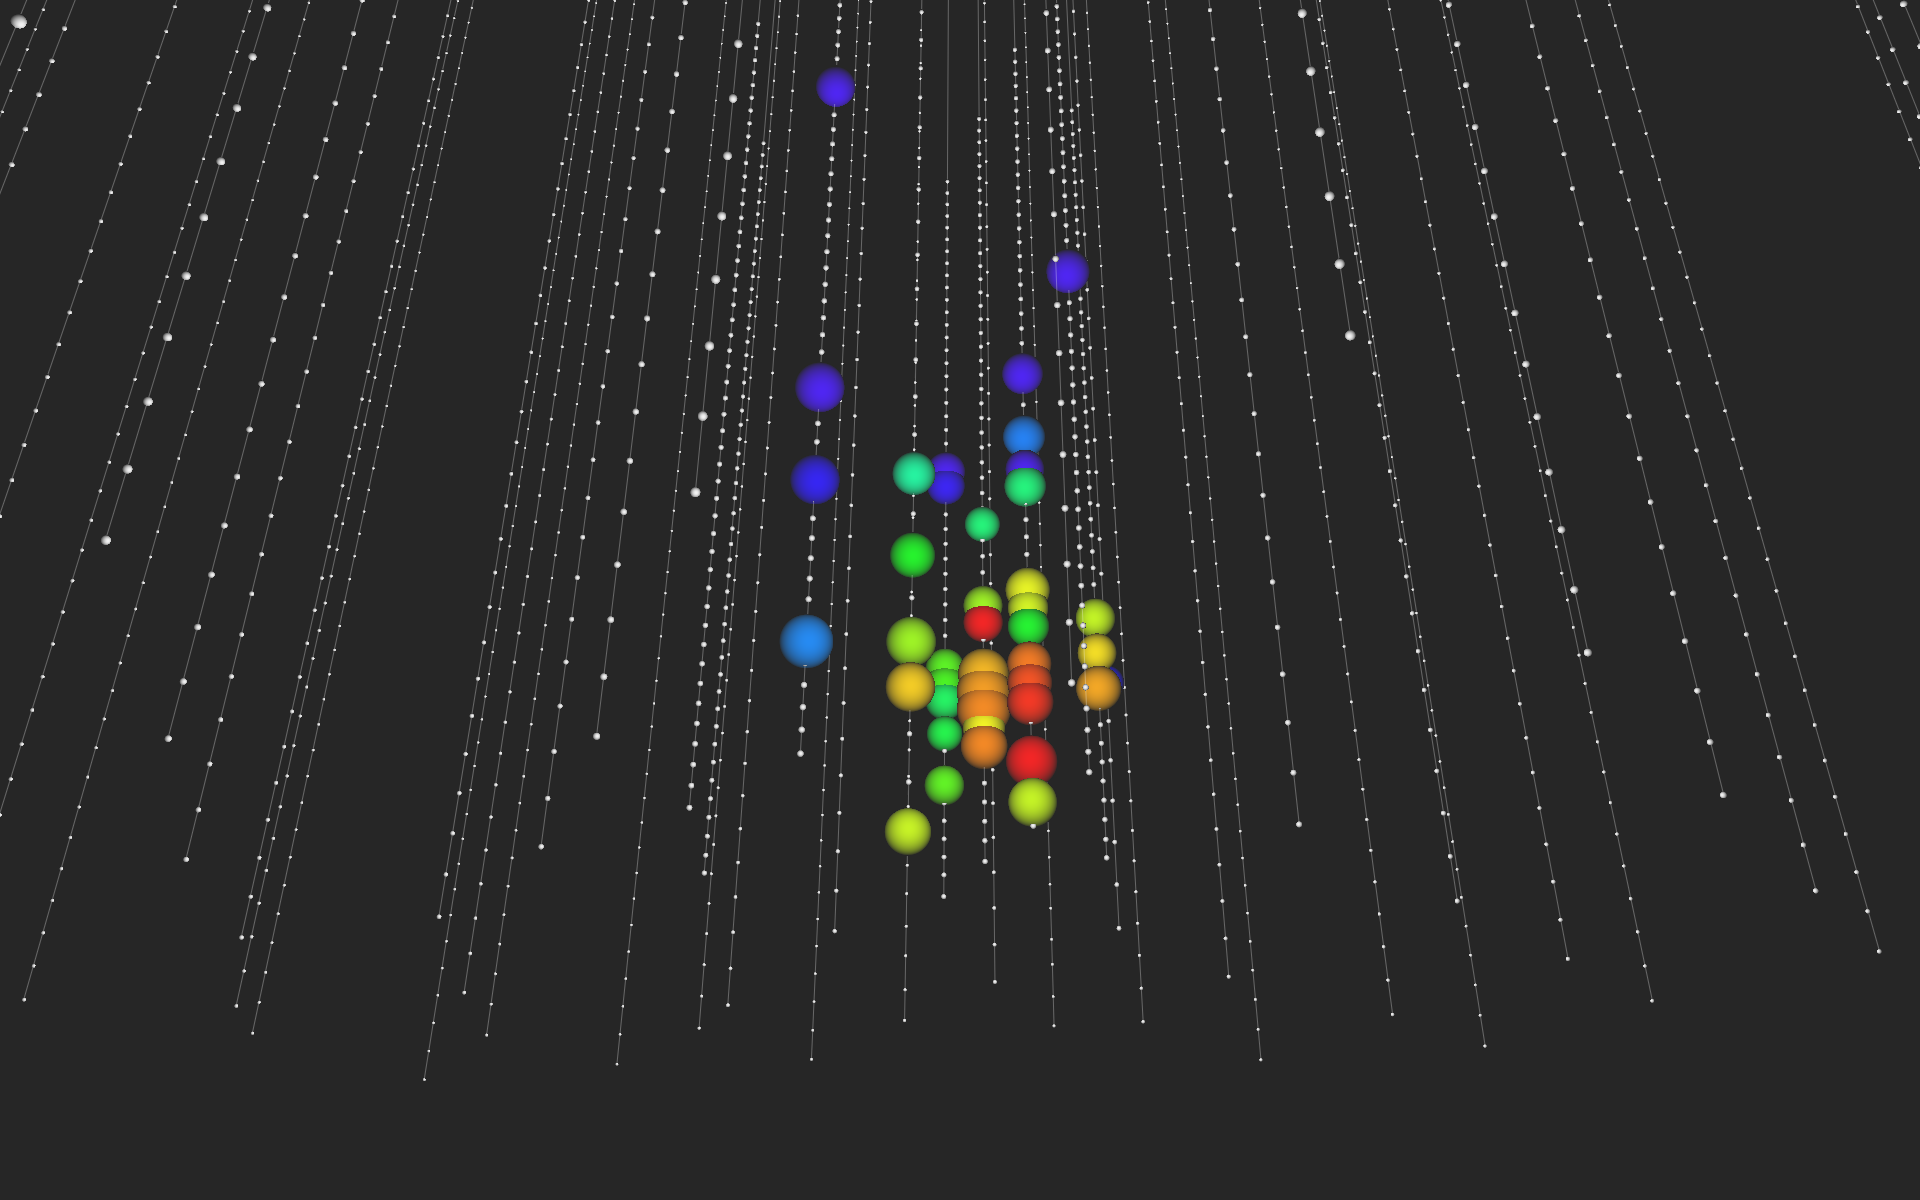
\includegraphics[trim = 0 0 0 0, clip, width=0.45\linewidth]{figures/track_view_1.png}
        }
        \hspace{0.75cm}
        \subfloat[$\nu_e$-NC]{
        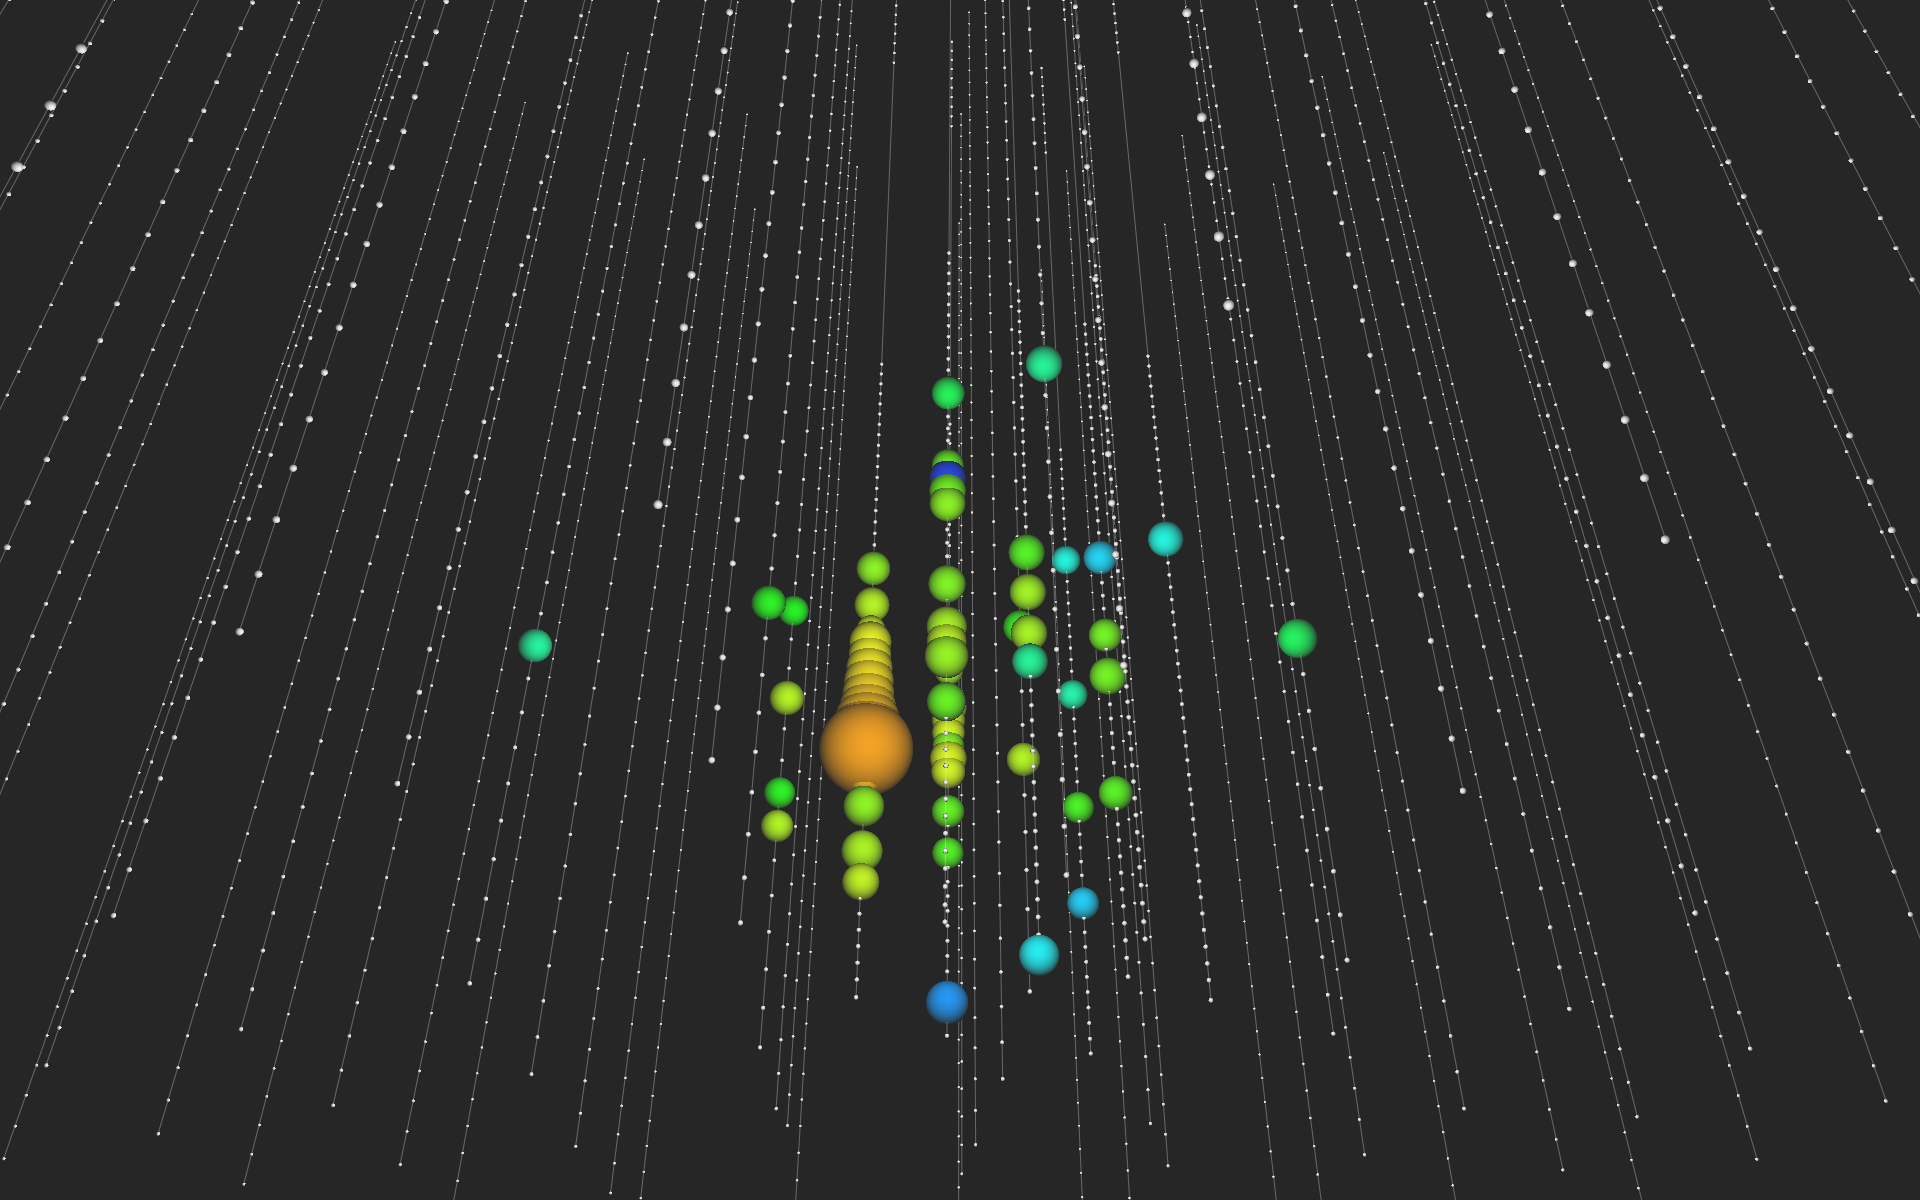
\includegraphics[trim = 0 0 0 0, clip, width=0.45\linewidth]{figures/cascade_view_1.png}
        }
    \caption[Examples of low energy track and cascade events]
    {Examples of low energy track and cascade events. The color of the spheres indicates the signal time, where red is early and blue is late. Their size is proportional to the integrated charge in each DOM. The depicted events have a neutrino energy of $\mathcal{O}$(GeV).}
    \label{fig:topologies_low_energy}
\end{figure}

In previous works, a single reconstructed variable was used as a PID discriminator.
Here instead several variables are used to train a multivariate machine learning algorithm to find a more powerful PID discriminator.
Section~\ref{sec:interesting_variables} introduces a selection of relevant reconstructed variables.
Section~\ref{sec:gradient_boosting_classifier} presents the multivariate method and Section~\ref{sec:classifier_results} shows the results of the classification.


\section{Reconstructed Variables} \label{sec:interesting_variables}

The main motivation for the work done in this thesis is the number of reconstructed quantities that might be useful in discriminating event signatures between tracks and cascades.
All variables are taken from the event reconstruction outlined in Section~\ref{sec:event_reconstruction}.
Figure~\ref{fig:feature_distributions} shows the distributions of selected variables, split in $\nu_\mu$-CC (track) and $\nu_e$-CC+$\nu_e$-NC+$\nu_\mu$-NC (cascade).

\begin{figure}[h] 
    \centering
    \subfloat[$\chi^2\textrm{-ratio}$]{ \label{fig:feature_distributions_a}
    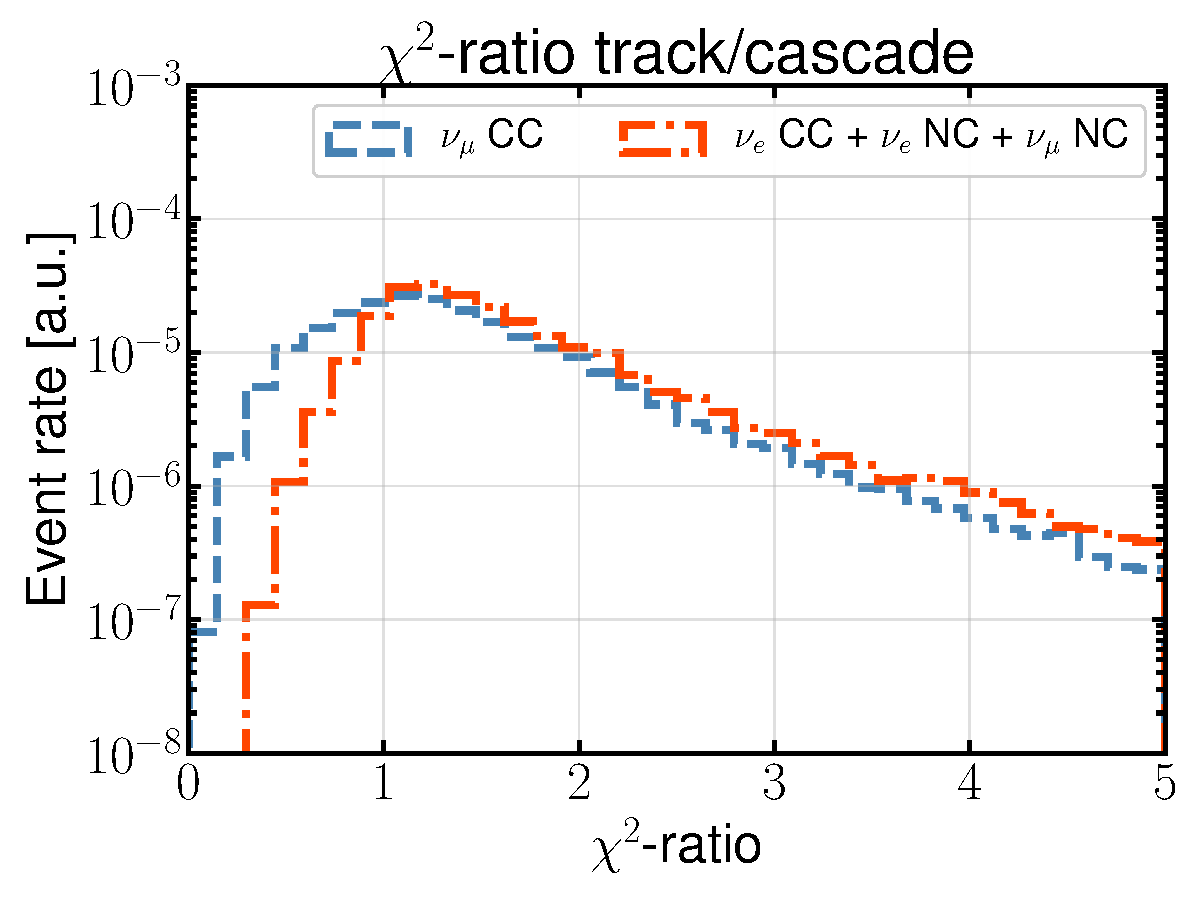
\includegraphics[width=0.31\linewidth]{figures/santa.pdf}
    }
    \subfloat[Track length]{ \label{fig:feature_distributions_b}
    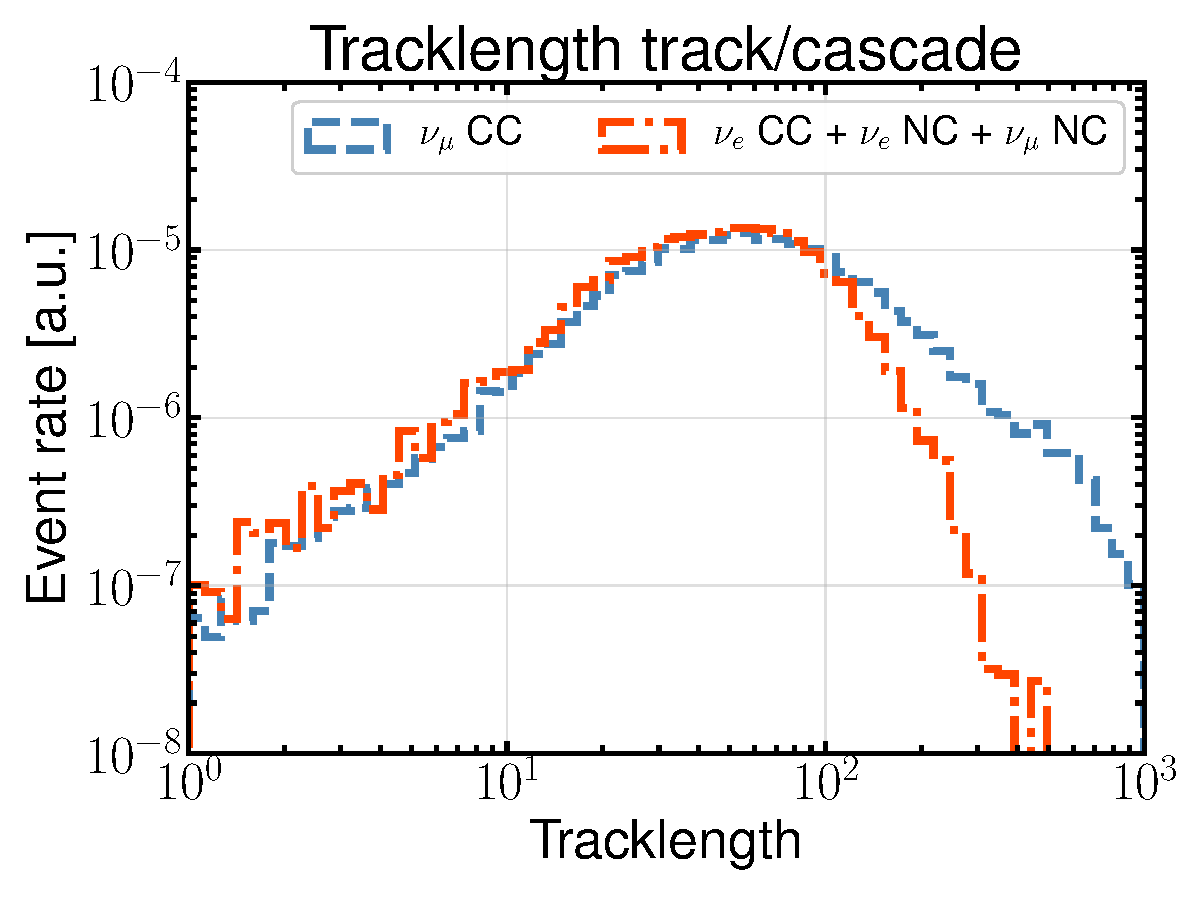
\includegraphics[width=0.31\linewidth]{figures/tracklength.pdf}
    }
    \subfloat[LLH-difference]{  \label{fig:feature_distributions_c}
    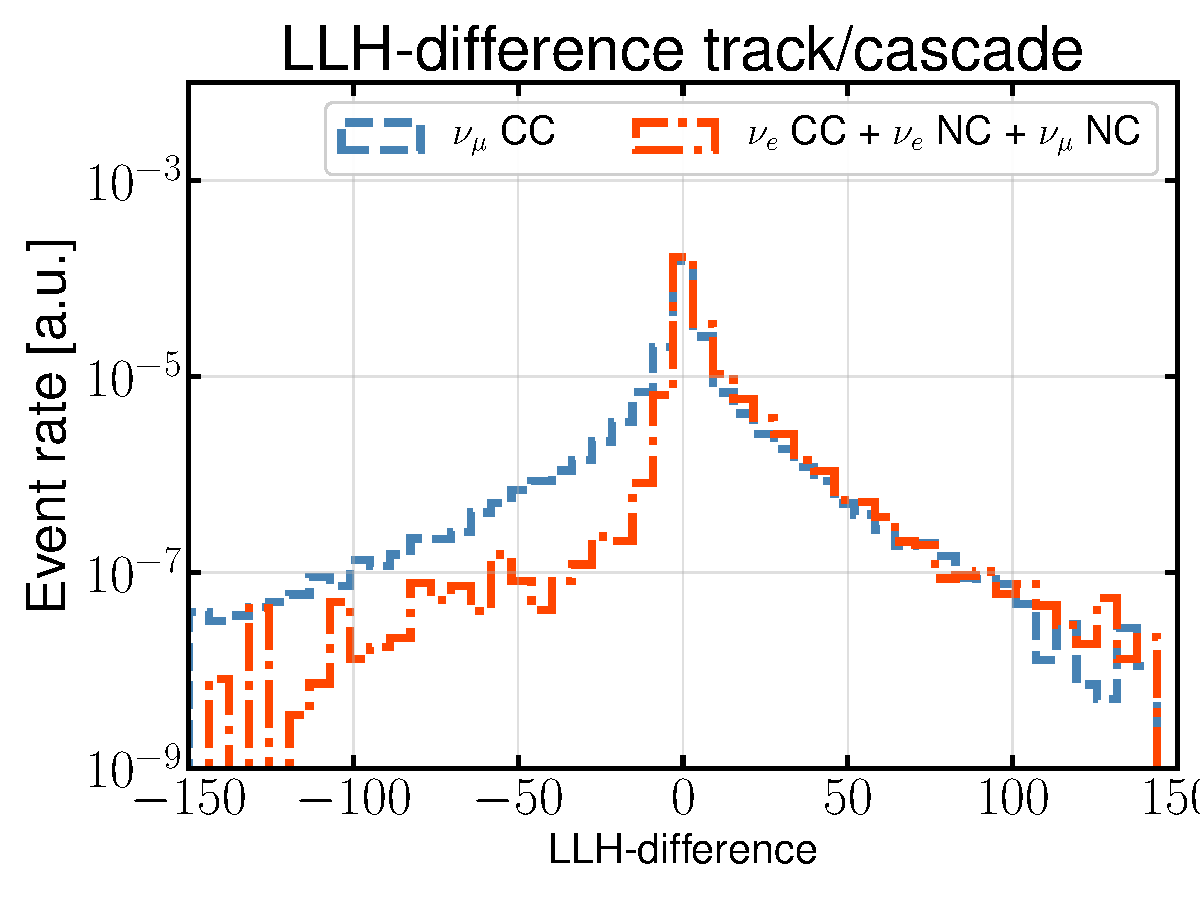
\includegraphics[width=0.31\linewidth]{figures/leera.pdf}
    }
    
    \subfloat[Vertex radius]{ \label{fig:feature_distributions_d}
    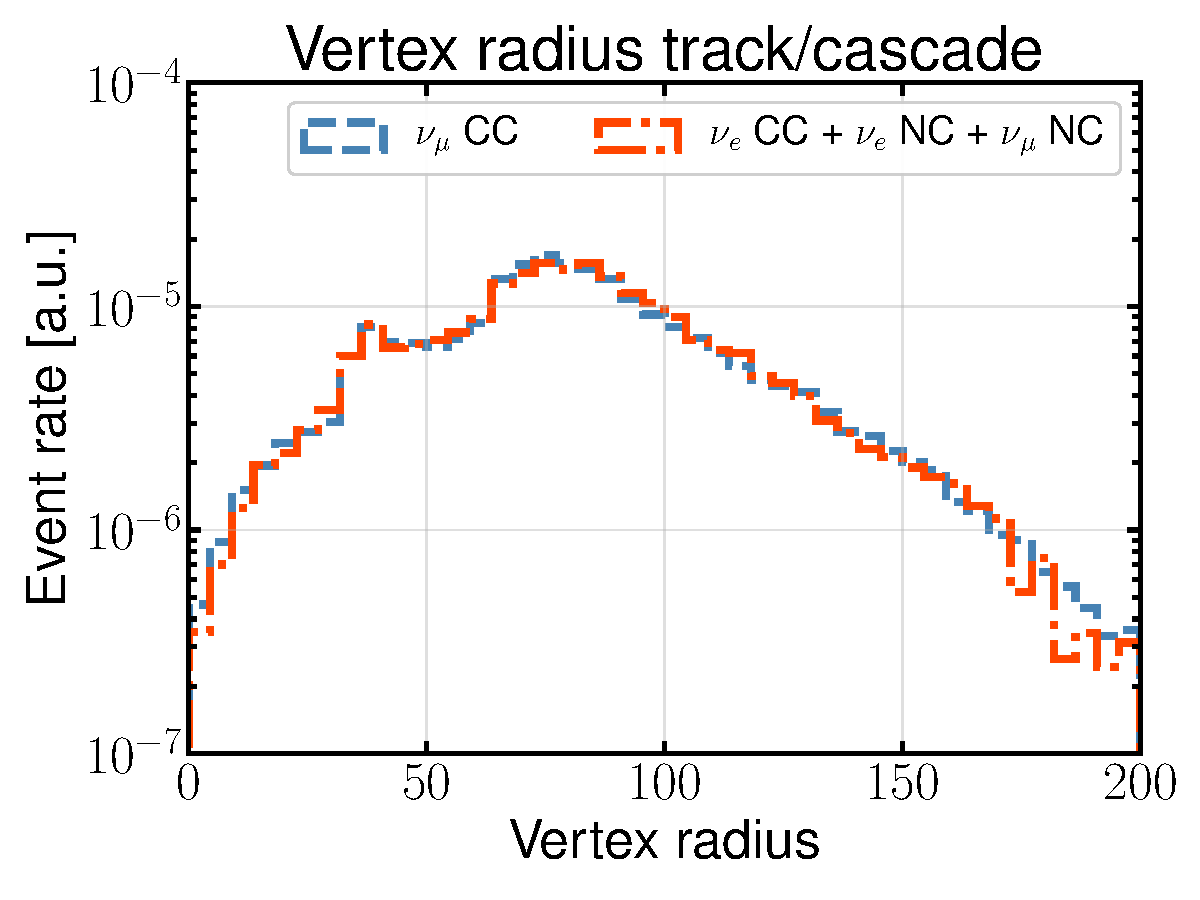
\includegraphics[width=0.31\linewidth]{figures/rho36_start.pdf}
    }
    \hspace{.5cm}
    \subfloat[Endpoint radius]{ \label{fig:feature_distributions_e}
    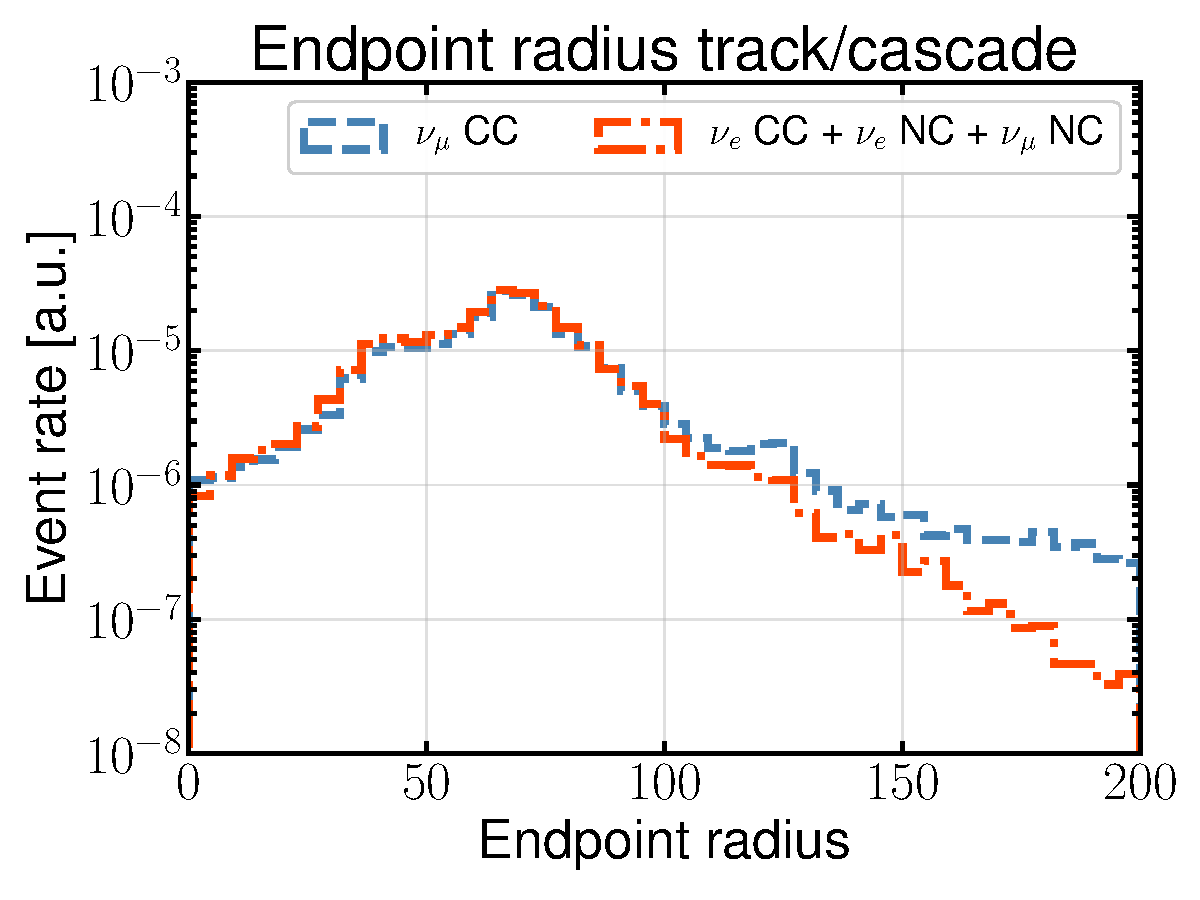
\includegraphics[width=0.31\linewidth]{figures/rho36_end.pdf}
    }
    
    \subfloat[Vertex depth]{ \label{fig:feature_distributions_f}
    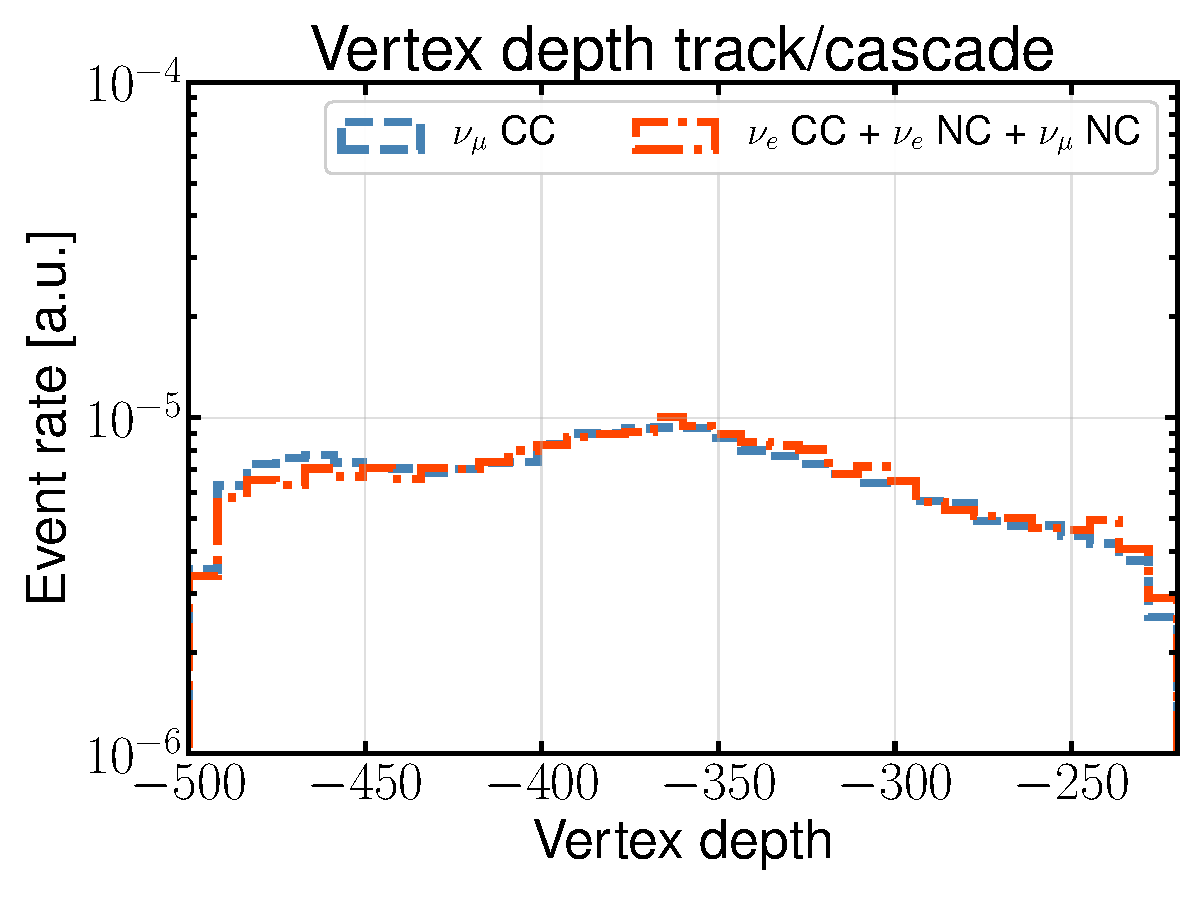
\includegraphics[width=0.31\linewidth]{figures/z_start.pdf}
    }
    \hspace{.5cm}
    \subfloat[Endpoint depth]{ \label{fig:feature_distributions_g}
    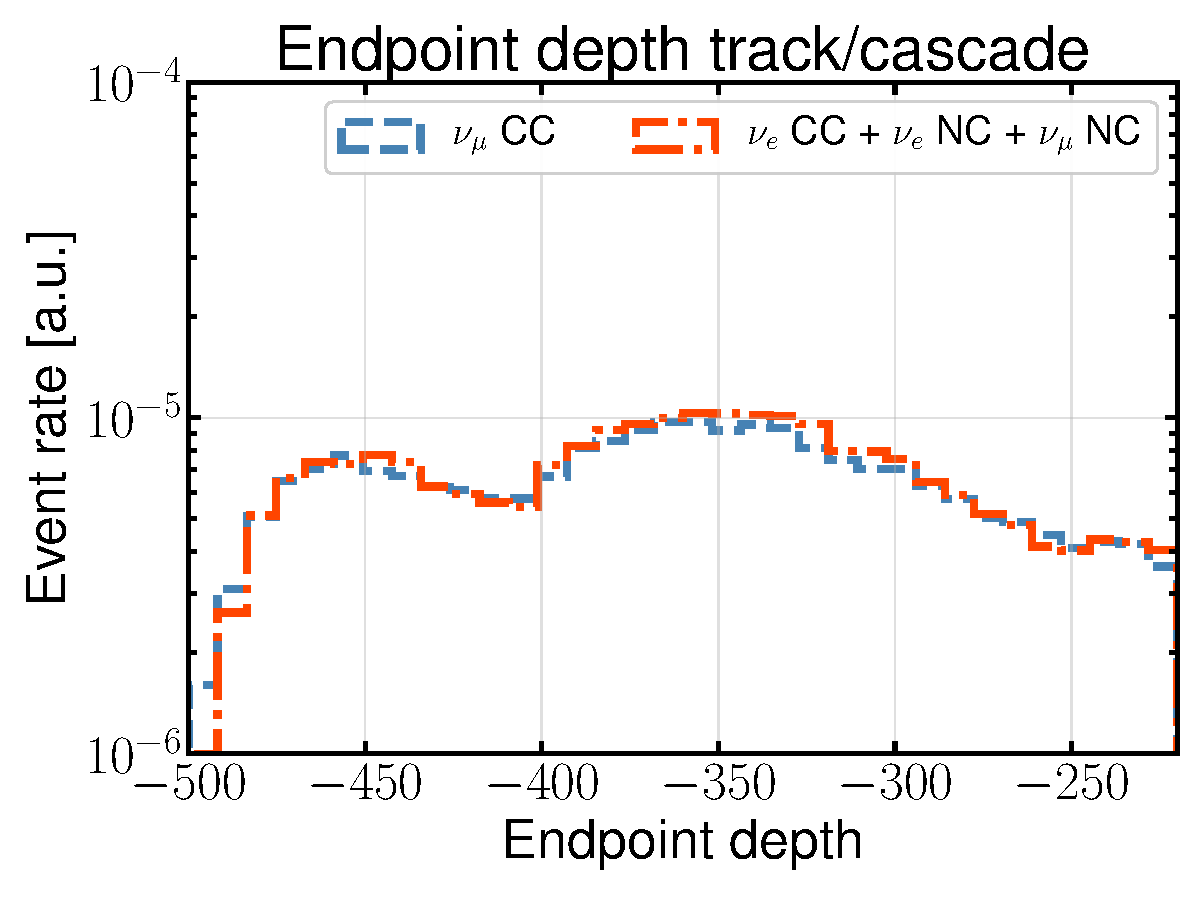
\includegraphics[width=0.31\linewidth]{figures/z_end.pdf}
    }
    \caption[Distributions of the selected input features]{Distributions of the selected input features split in $\nu_\mu$-CC (track) and $\nu_e$-CC+$\nu_e$-NC+$\nu_\mu$-NC (cascade) events. The rates are scaled to the same area so that the shapes can be compared.}
    \label{fig:feature_distributions}
\end{figure}

Two of these variables are related to the fit performance of the event reconstruction, while the rest of them are reconstructed physical quantities themselves.
The first interesting variable that was used as a PID variable in previous analyses \cite{2017arXiv170205160I, ATerliuk} is the ratio between the goodness of fit for a track hypothesis and a cascade hypothesis in the directional reconstruction explained in \ref{sec:directional_reconstruction}.
The variable referred to as the $\chi^2\textrm{-ratio}$ (Figure~\ref{fig:feature_distributions_a}) is calculated as
\begin{equation}
    \chi^2\textrm{-ratio} = \frac{\chi^2_\mathrm{track}}{\chi^2_\mathrm{cascade}}\cdot\frac{\mathrm{DoF}_\mathrm{cascade}}{\mathrm{DoF}_\mathrm{track}},
\end{equation}
where $\mathrm{DoF}_\mathrm{cascade}$ and $\mathrm{DoF}_\mathrm{track}$ are the degrees of freedom in the respective fit.
They are $\mathrm{DoF}_\mathrm{cascade} = \mathrm{N}_\mathrm{DOMs}-3$ and $\mathrm{DoF}_\mathrm{track}=\mathrm{N}_\mathrm{DOMs}-4$.
$\mathrm{N}_\mathrm{DOMs}$ is the number of DOMs with direct photons used for the reconstruction.
Small values of the $\chi^2\textrm{-ratio}$ indicate track-like events and large values cascade-like events.
This behavior can clearly be seen in Figure~\ref{fig:feature_distributions_a}.

Another variable, which is related to the energy reconstruction described in Section~\ref{sec:energy_reconstruction}, is the difference of negative log-likelihoods (compare Equation~\ref{eq:track_no_track_LLLHR}) for the track- and cascade-only hypothesis fit, defined as
\begin{equation}
    \textrm{LLH-difference} = \textrm{LLH}_\mathrm{track}\textrm{ - LLH}_\mathrm{cascade}.
\end{equation}
Since small LLH values imply a good fit, small values of the LLH-difference (Figure~\ref{fig:feature_distributions_c}) suggest track-like events and large values cascade-like events.
Figure~\ref{fig:feature_distributions_c} shows the indicated behavior of the LLH-difference.

The other features are related to the reconstructed position of the interaction vertex and the reconstructed track length.
The track length (Figure~\ref{fig:feature_distributions_b}) itself also holds potential in discriminating tracks from cascades, as can be seen in Figure~\ref{fig:feature_distributions_b}.
Events from $\nu_\mu$-CC interactions (tracks) have longer reconstructed track lengths than events coming from $\nu_e$-CC+$\nu_e$-NC+$\nu_\mu$-NC interactions (cascades).
This is especially true for higher energy $\nu_\mu$-CC interactions where the muon carries a large amount of energy.
Figure~\ref{fig:feature_distributions} also shows the horizontal, radial distance to the center of the detector for the interaction vertex (Figure~\ref{fig:feature_distributions_d}) and the track endpoint (Figure~\ref{fig:feature_distributions_e}) as well as the depth of the two positions (Figure~\ref{fig:feature_distributions_f}, Figure~\ref{fig:feature_distributions_g}).
The position of the endpoint of the track combines the information of the direction of the event and the reconstructed track length from the energy reconstruction.
It seems like these variables are not useful in discriminating tracks from cascades, because the track and cascade distributions are very similar.
This is certainly true when using them as a single discriminator, but in combination with other variables by applying a multivariate technique they are useful.
This will be further discussed in Section~\ref{sec:feature_selection}.
Another reason why the spatial variables are used is that the instrumentation of IceCube is much denser around the center as shown in Figure~\ref{fig:icecube_top_view}.
As a result, the reconstruction performs better in the center leading to more accurate reconstructed quantities.
This could improve the classification for events occurring in the that region.


\section{Gradient Boosting Classifier} \label{sec:gradient_boosting_classifier}

As already mentioned, the goal is to develop a new event classification algorithm for PID.
As discussed in Section~\ref{sec:interesting_variables}, there are multiple variables that hold some separation power between tracks and cascades.
But, since there is no direct functional relation between these variables and the neutrino flavor, we need to build a non-parametric classification model.
For this purpose, we utilize the Monte-Carlo (MC) simulation of IceCube events that is available.
There are a variety of ways to build a multivariate model.
Here we choose to apply a Gradient Boosting Machine (GBM) \cite{friedman2001}.

GBMs are machine learning techniques that combine weak prediction models in a stage-like fashion to produce a strong prediction model.
GBMs can be used to optimize any differentiable loss function and offer the possibility to tune the parameters of the training process for custom use.
In this work, we use the Gradient Tree Boosting algorithm provided by the scikit-learn package \cite{scikit-learn}.
In this case, the weak prediction models are formed by simple decision trees, which are models that predict a discrete output variable dependent on a set of input variables.
Figure~\ref{fig:example_decision_tree} shows a visualization of an example decision tree.
Following the paths from the root at the top to the leaves at the bottom, at every interior node the data is split by applying a straight cut on one of the input variables.
The cuts are chosen to achieve the best possible separation of the data into the output classes, measured by some metric.
The cuts and the variables are specified at the top of each node.
Also shown is the percentage of the sample chosen by the applied cuts.
Each leaf provides a value for the output variable dependent on the input variables.
The different paths from the root to the leaves form the classification rules.
Figure~\ref{fig:example_decision_tree} shows what fractions are tracks and cascades and a classification into the output classes, based on the class of the majority of events.
The boosting algorithm fits multiple such decision tree models in an iterative way, where at each step a loss function is calculated from the ensemble of previously fit weak models.
The next decision tree will be constructed so that the ensemble loss is reduced along its negative gradient, leading to a reduction of the residual loss.
This process is repeated until the loss is reduced below a certain threshold or the maximum number of trees is reached.

\begin{figure}[h]
    \centering
    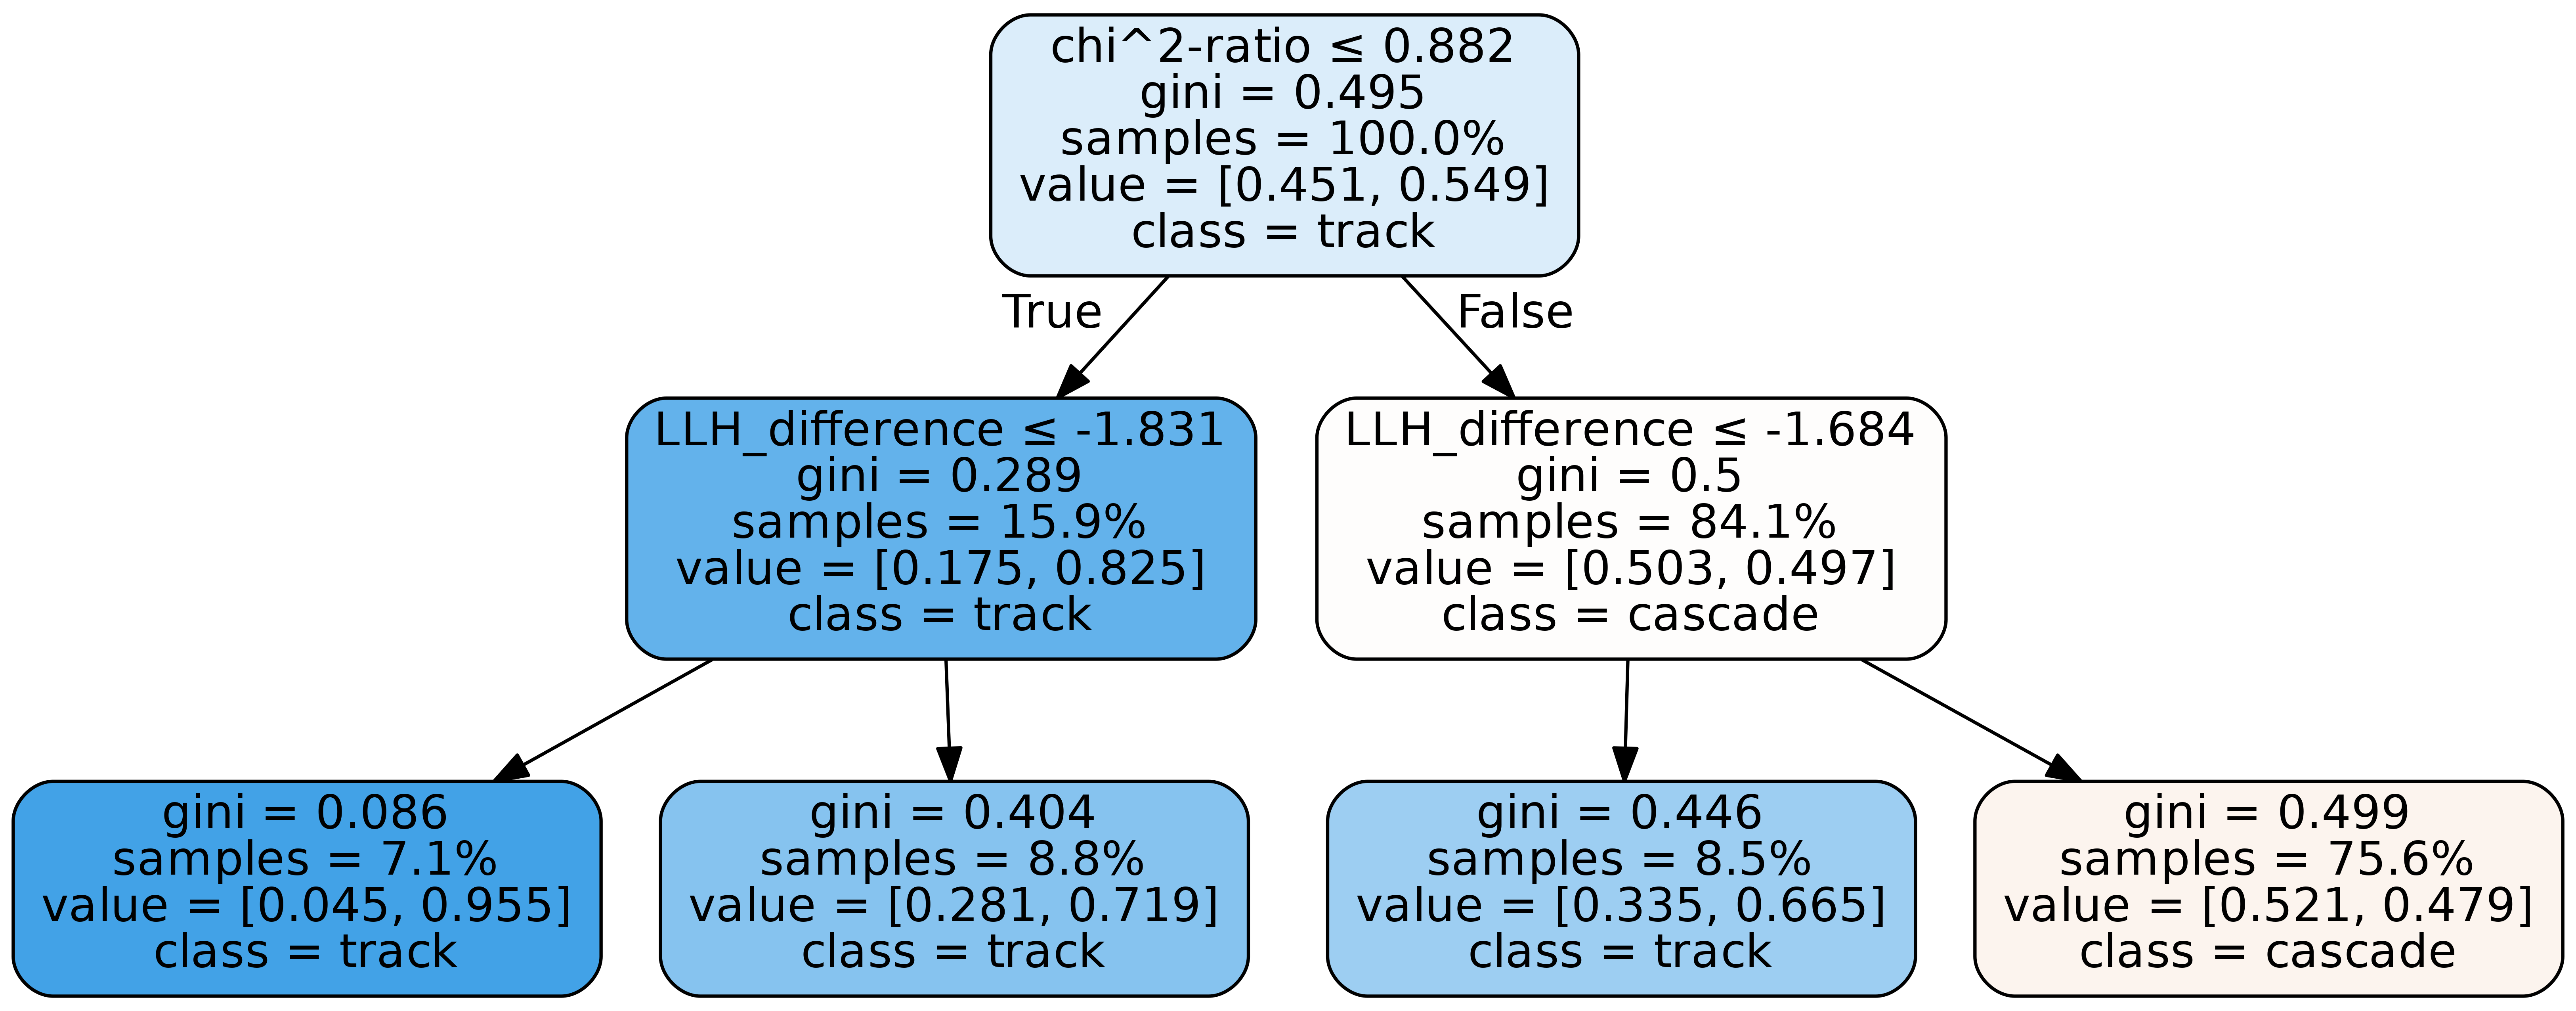
\includegraphics[align=b, trim = 00 00 00 00, clip, width=0.95\linewidth]{figures/example_tree.png}
    \caption[Example decision tree]{Example decision tree showing the variable and the chosen cut at the top of each node, the fraction of the full sample that is selected by each cut and the fractions that are track and cascade. Based on the bigger fraction a classification into track or cascade is displayed at the bottom of each node.}
    \label{fig:example_decision_tree}
\end{figure}

To use a GBM classifier on real data, we first need to train it on a dataset for which we know the true interaction type.
For this work, the training is performed on a set of simulated neutrino events in the energy range of $1-1000$\,GeV.
To get a realistic distribution of events and to take into account the atmospheric neutrino production explained in Section~\ref{sec:neutrino_atmospheric} and the detector volume, the events are weighted depending on their energy and direction.
The weights also include the oscillation probability, as will be discussed in Section~\ref{sec:likelihood_estimation}.
The units of the weights are chosen as events/s, such that summing over the weights of all events in a dataset gives the overall event rate.
The events are reconstructed using the methods explained in Section~\ref{sec:event_reconstruction}, but also carry the true information from the simulation production.
The following sections illustrate the process of selecting the input variables and performing some data pre-processing.


\subsection{Feature Selection} \label{sec:feature_selection}

The classifier is trained on a set of selected input variables.
These so-called \textit{features} are selected by investigating if they have some potential in separating tracks from cascades.

A first step is to check if the feature distributions for track and cascade vary significantly as already done in Section~\ref{sec:interesting_variables}.
Features that show a separation are useful to feed into a GBM, but features that do not can also be useful.

As a second step, we look at the Pearson correlations \cite{stigler1989} of the features.
The correlations for the selected features presented in Section~\ref{sec:interesting_variables} are shown in Figure~\ref{fig:feature_correlations}.
Again, they are split in $\nu_\mu$-CC (track) and $\nu_e$-CC+$\nu_e$-NC+$\nu_\mu$-NC (cascade).
\begin{figure}[h]
    \centering
    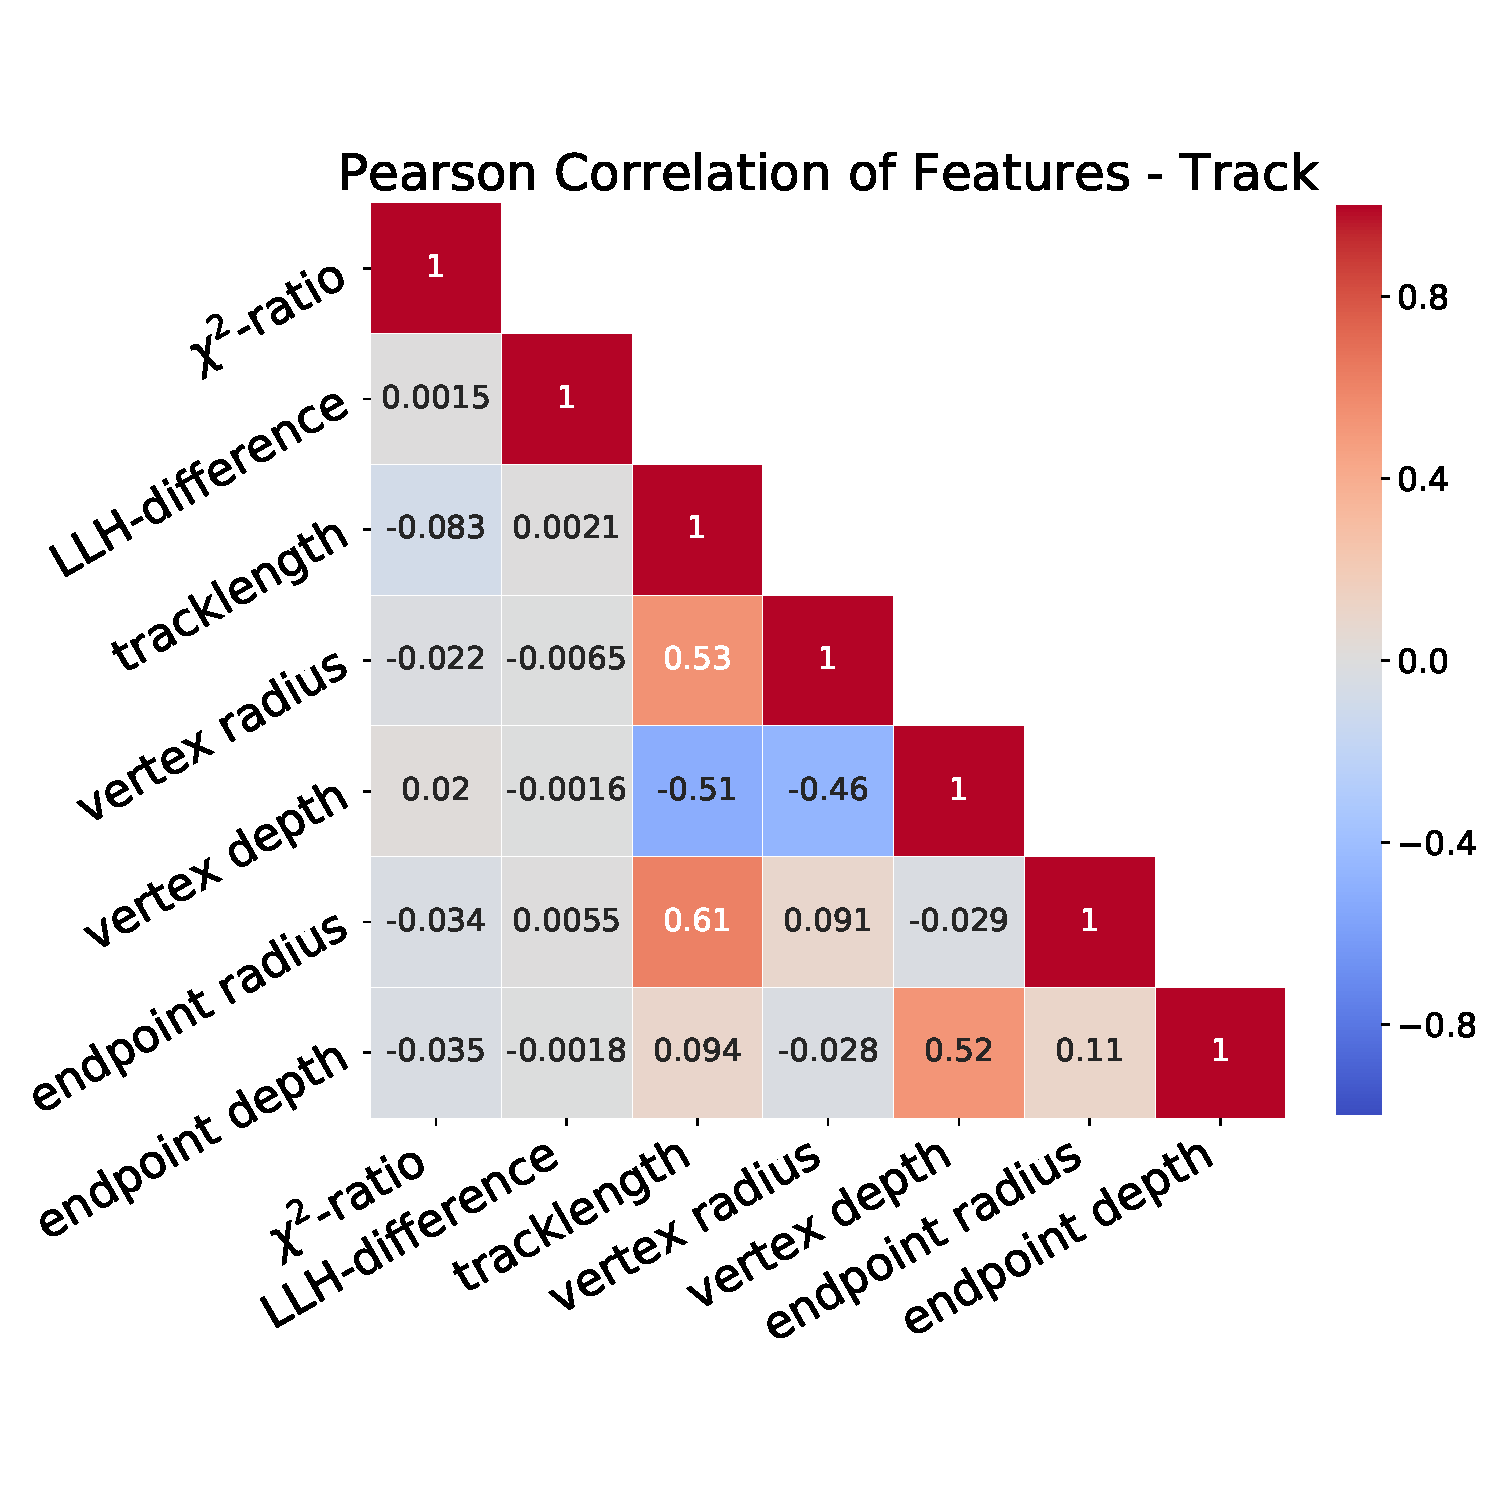
\includegraphics[trim = 10 70 10 65, clip, width=0.49\linewidth]{figures/feature_correlations_Track.pdf}
    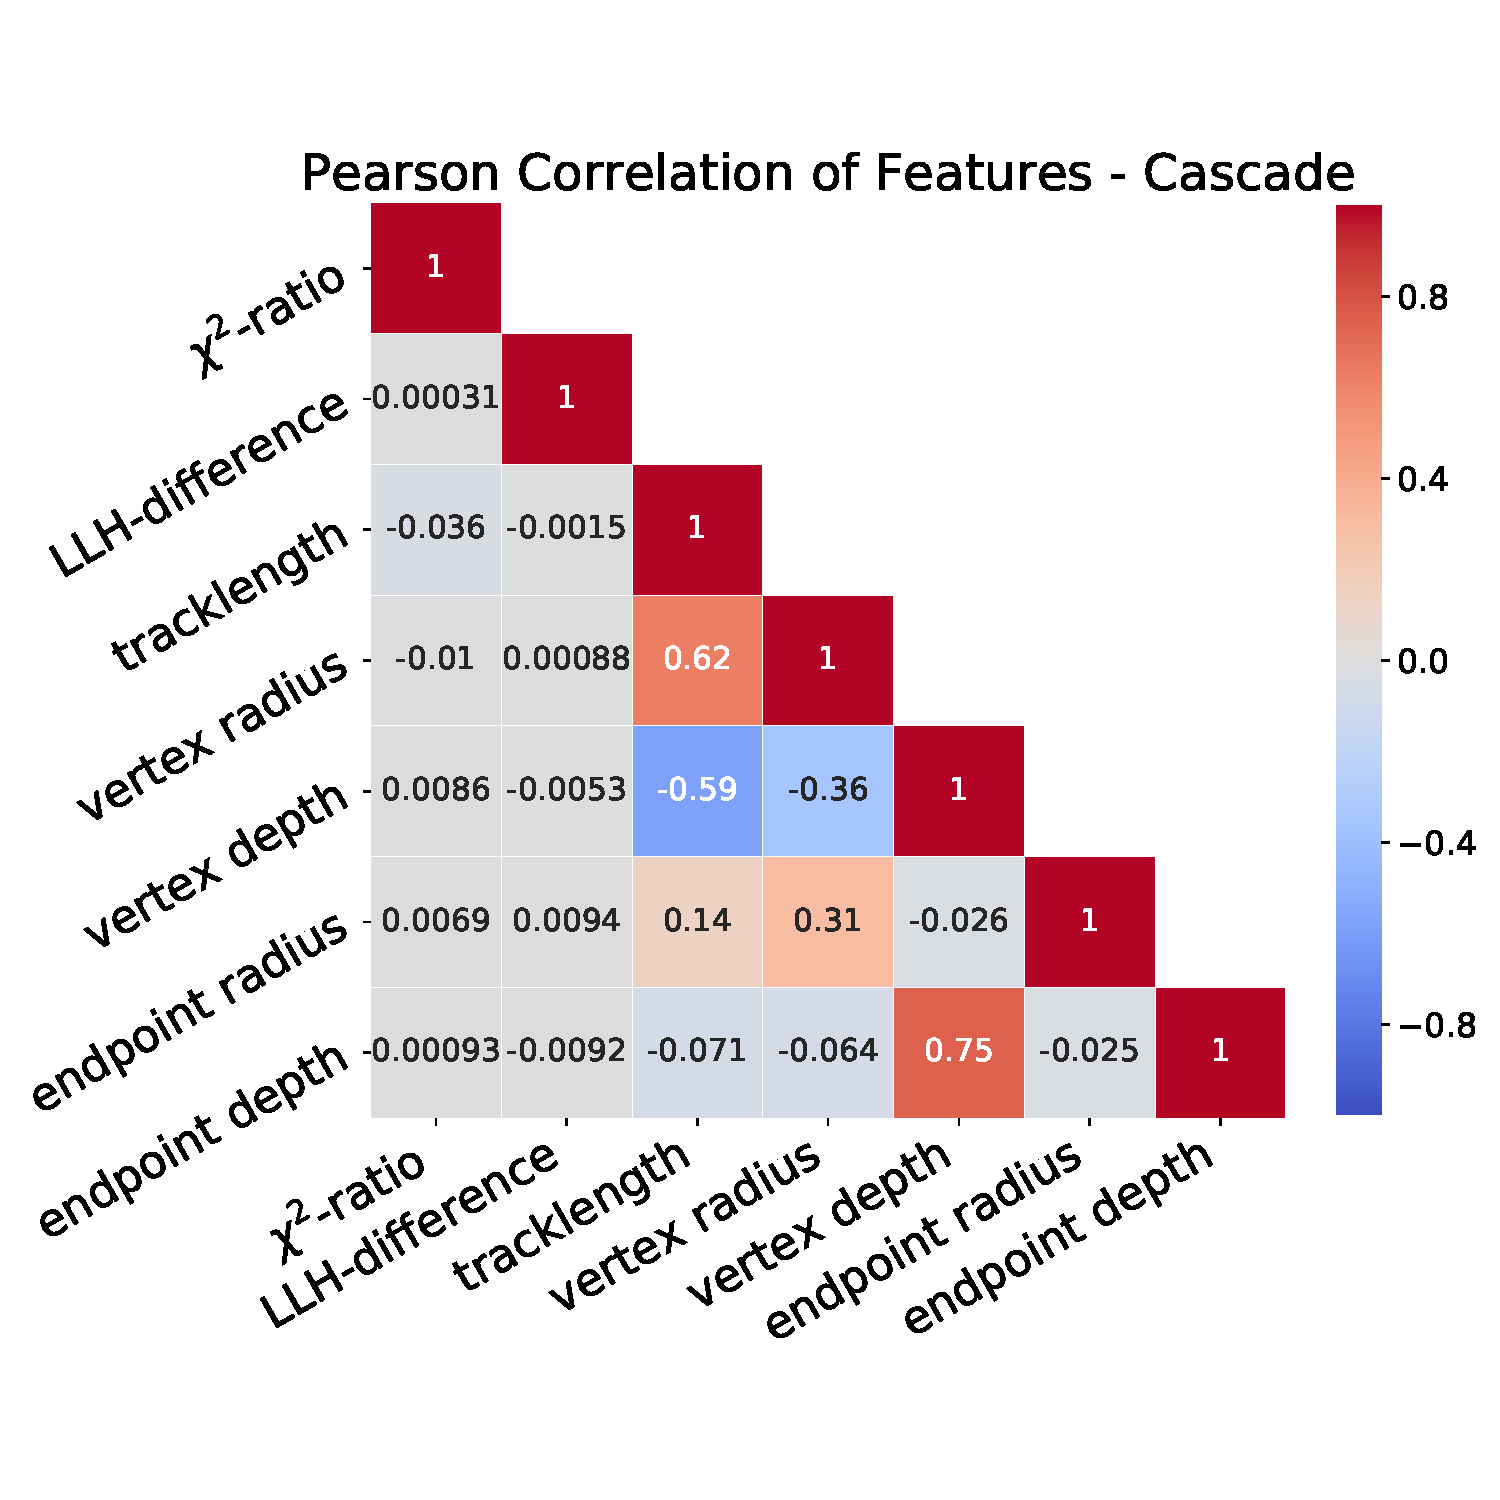
\includegraphics[trim = 10 70 10 65, clip, width=0.49\linewidth]{figures/feature_correlations_Cascade.pdf}
    \caption[Pearson correlation of the selected input features]{Pearson correlation of the selected features for $\nu_\mu$-CC (track-like) events (left) and $\nu_e$-CC+$\nu_e$-NC+$\nu_\mu$-NC (cascade-like) events (right). The color code indicates the strength of the correlation.}
    \label{fig:feature_correlations}
\end{figure}
Features can help the classification if their correlations with other features are different for tracks and cascades.
For example, we see that for tracks the correlation between track length and $\chi^2\textrm{-ratio}$ is -0.083, while for cascades it is only -0.036.
Also interesting are correlations between features that show a strong separation in track and cascade and features that do not.
For example, with a value of 0.00093, there is effectively no correlation between the $\chi^2\textrm{-ratio}$ and the track endpoint depth for cascades but for tracks the correlation is -0.035.

As a third step, we need to guarantee that the classification based on the features will perform in the same way when applied to real data.
Although the MC simulation set reflects the current best knowledge of the neutrino interactions and fluxes as well as the detector properties, there could still be inaccuracies.
This could lead to a mismatch between variable distributions in data and simulation as well as wrong correlations between the variables.
We therefore check if the feature distributions agree between data and simulation.
For the purpose of checking the agreement, 10\,\% of the data of the years 2011-2018 are used and a larger MC dataset.
The weights are calculated assuming standard oscillations with $\Delta\mathrm{m}^2_{32}=2.42\cdot10^{-3}$\,eV$^2$ and sin$^2\theta_{23}=0.538$.
The detailed comparison plots for every feature variable are listed in appendix~\ref{app:data_mc_checks}.
The agreement is reasonable for all of the features.
It should be noted that this comparison is done without having performed a fit on the oscillation parameters and the overall normalization.

Finally, the selection of input features is determined after checking the performance of the classifier depending on some chosen metric.
The importances of the individual features can be extracted for a trained classifier.
This shows which of the features has the strongest effect on the classification.
Based on the importances, features can be removed and new feature combinations tested.
The set of features that results in the best performance is chosen.
The features discussed here are the best combination found and, therefore, the selection chosen in this work.


\subsection{Data Preprocessing}

To prepare the data for the training, some pre-processing steps are necessary.
Only events that passed the directional reconstruction cleaning procedure will have the features chosen for the training and in some cases the energy reconstruction fails even though the directional reconstruction succeeded.
For this reason, all events are removed where some of the features are missing.
After removing these incomplete events, a boolean variable is created indicating whether the event is a true track ($\nu_\mu$-CC) or a true cascade ($\nu_e$-CC+$\nu_e$-NC+$\nu_\mu$-NC).
This boolean variable will be used as a target variable for the training step.
Events coming from any $\nu_\tau$ interaction are not taken into account here, because to first order they are true cascades.
For the training step the $\nu_\tau$ weights are, therefore, set to zero.
The training of the classifier is always performed on a subsample of the data called the \textit{training set}, while the remaining part of the data - called the \textit{test set} - is used to estimate its performance and test its robustness. 
In this thesis, the data is split in $\sim$50\,\% training set and $\sim$50\,\% test set.
To compensate for the fact that there are significantly more track-like events in the sample than there are cascade-like events, the weights of the events are scaled in a way so that the total rate of tracks and cascades is the same.
Additionally, the weights of all events are scaled to lie between 0 and 1.
Otherwise, the classifier can struggle to handle very small numerical values.


\section{Classifier Results} \label{sec:classifier_results}

The results of the best-performing classifier are reported here.
For every event that is classified by the trained algorithm, a probability score is calculated that represents the probability to be a true track event.
Figure~\ref{fig:bdt_probability_distribution} shows the probability score distribution for training and test sets split in $\nu_\mu$-CC (tracks) and $\nu_e$-CC+$\nu_e$-NC+$\nu_\mu$-NC (cascades).
\begin{figure}[h]
    \centering
    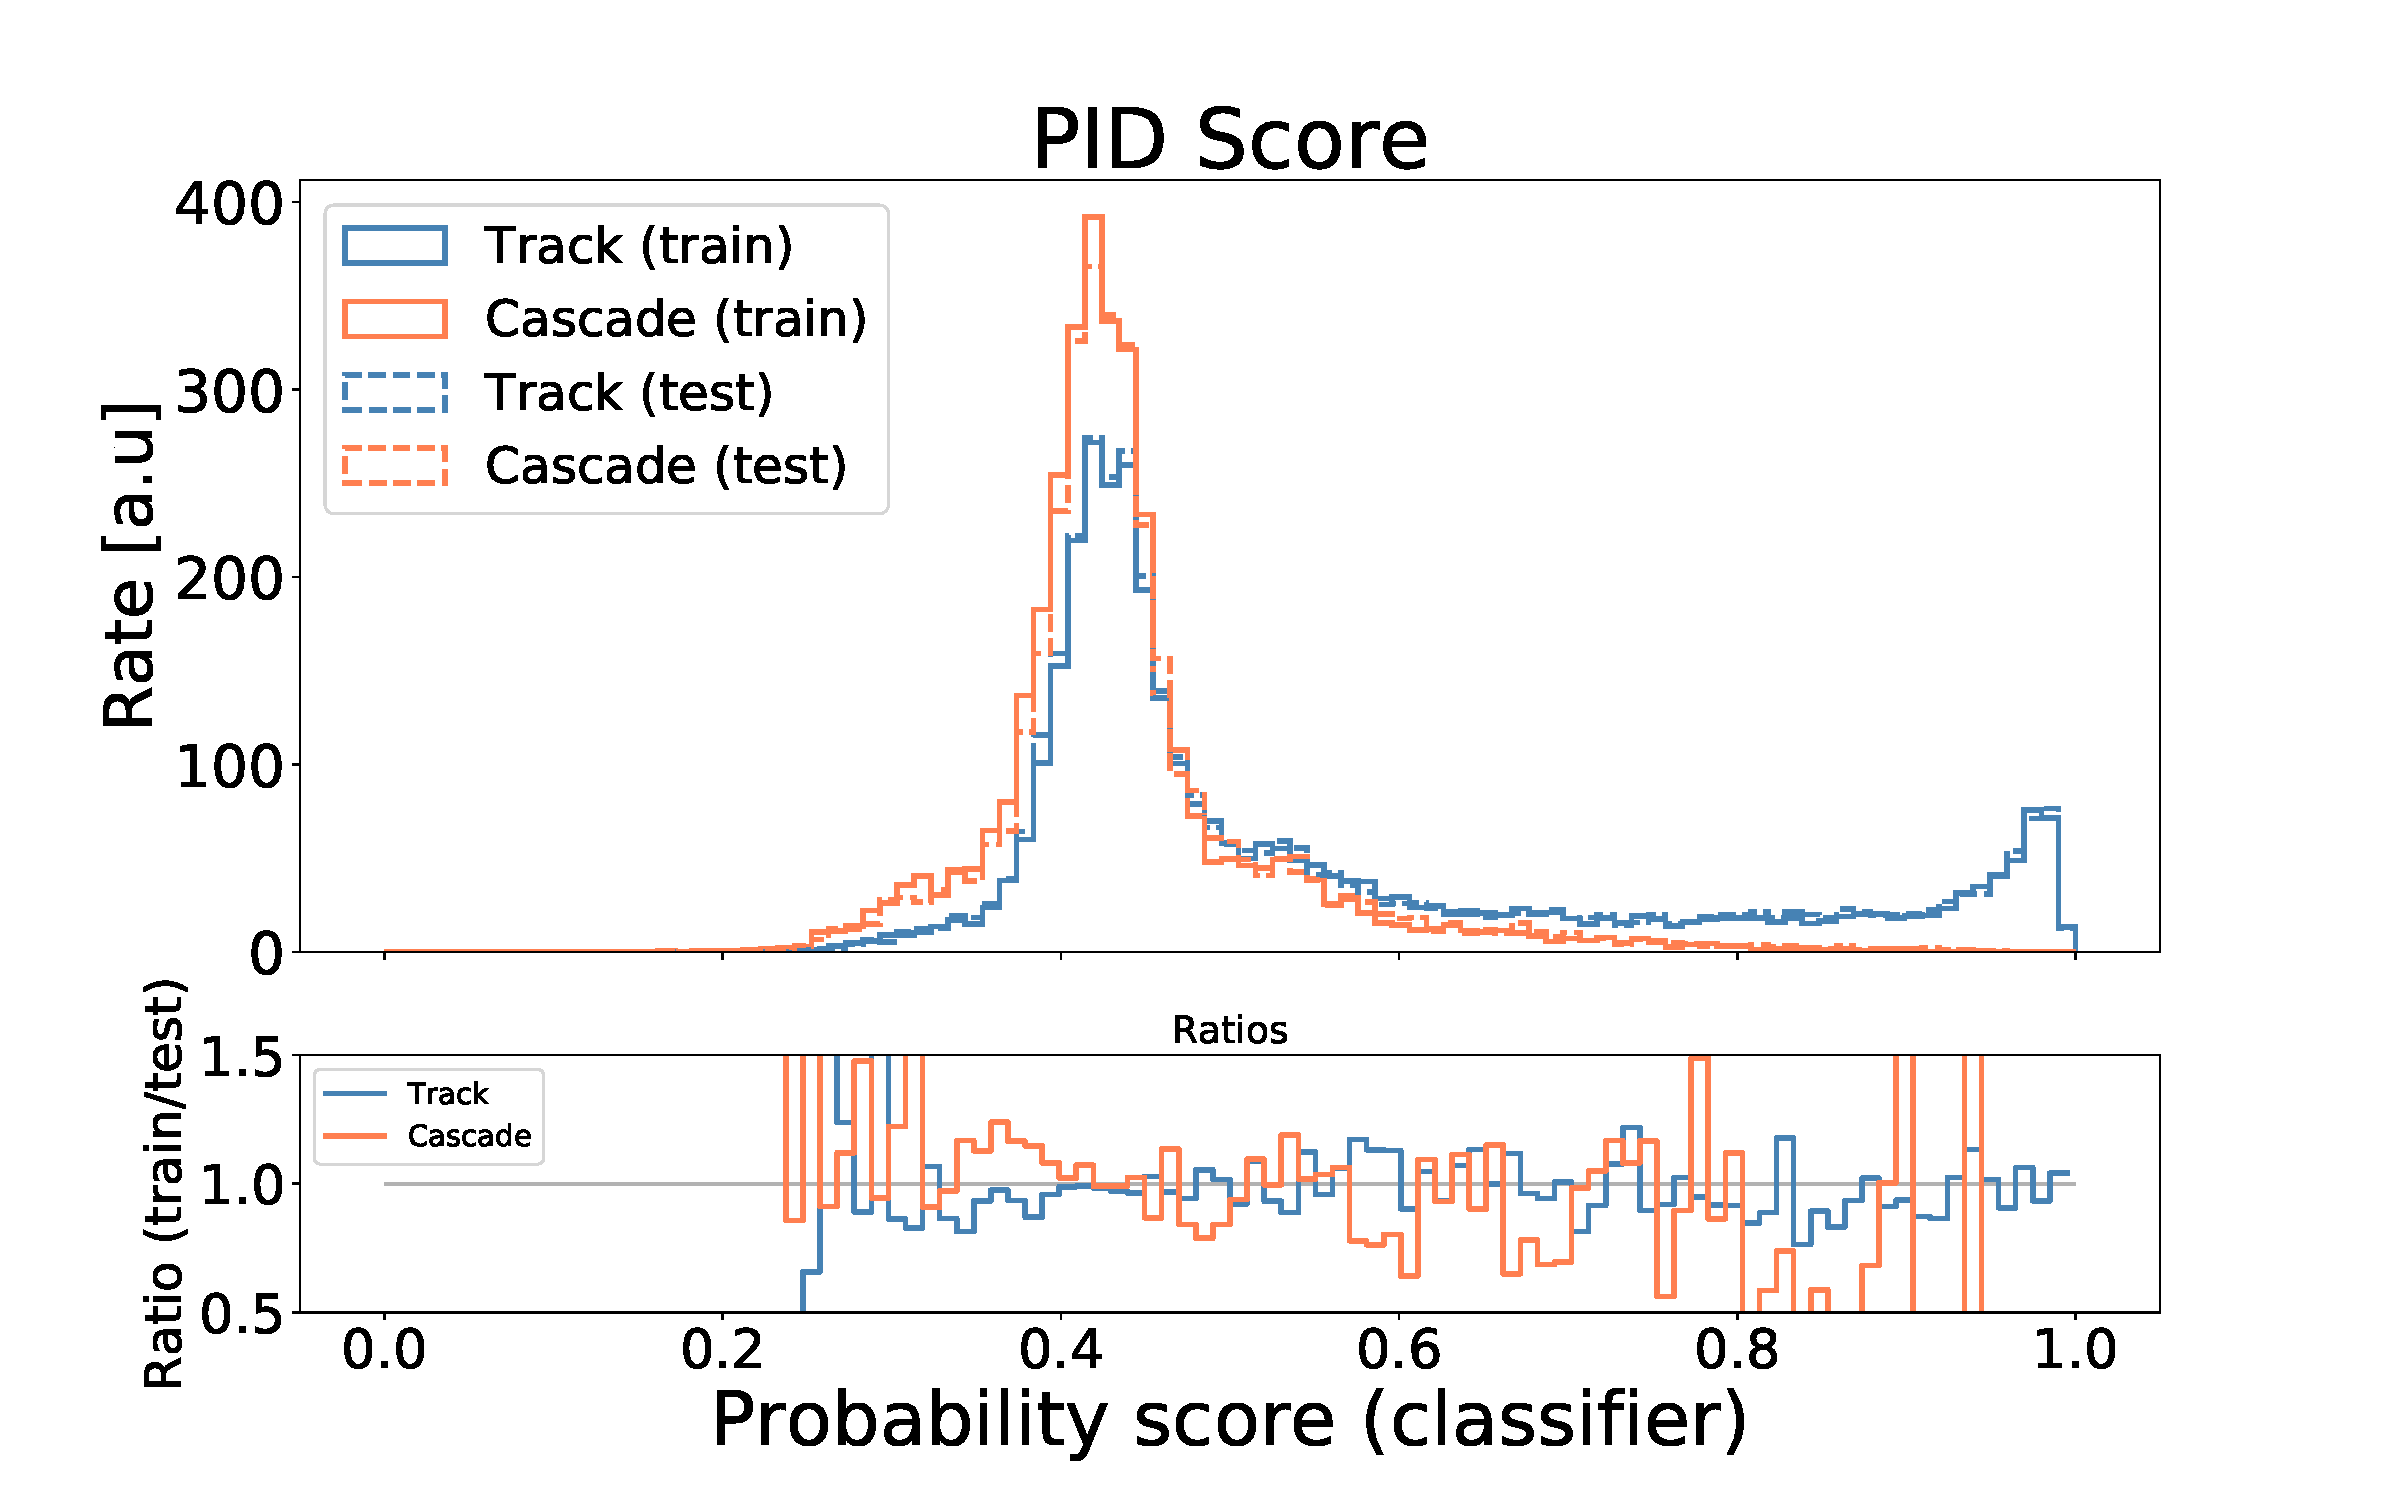
\includegraphics[trim = 35 05 110 25, clip, width=1.0\linewidth]{figures/probability_distribution.pdf}
    \caption[Classifier output probability of final, trained classifier]{Classifier output probability of the final, trained classifier for training/test set split in $\nu_\mu$-CC (track) and $\nu_e$-CC+$\nu_e$-NC+$\nu_\mu$-NC (cascade).}
    \label{fig:bdt_probability_distribution}
\end{figure}
There is a clear peak at values close to 1, which indicates track-like events.
For lower probability scores the cascades dominate the distribution, but there is still a significant track population.
These events are not separated very efficiently by the classifier.
Based on the probability distribution, we can divide events into subsamples that are track- and cascade-dominated.
Historically, there have only been two bins, but in principle any number of PID bins could be chosen.
The bins are selected by applying cuts to the probability distribution.
Ultimately, the optimal cut values will depend on the explicit analysis being performed.
As a test case, we consider the impact this classifier has on the sensitivity to atmospheric neutrino oscillations in Chapter~\ref{chap:oscillation_parameter_measurement}.
Several cut values and number of PID bins are tested for this type of analysis.

The receiver operating characteristic curve (ROC curve) of the trained classifier is shown in Figure~\ref{fig:roc_curve} compared to the ROC curve using only the $\chi^2$-ratio variable.
This graphical evaluation method is a visualization of how the probability score distribution for track and cascade is separated by straight cuts.
The curve shows the performance of the classifier for various thresholds, where the threshold is the cut on the probability score placed to split true and false (e.g. track and cascade).
As shown in Figure~\ref{fig:roc_curve} the true positive rate (TPR) is plotted on the y-axis against the false positive rate (FPR) on the x-axis.
TPR is the fractional number of correctly classified true events, while FPR is the fractional number of misclassified false events.
TPR, therefore, means the fraction of tracks that were correctly identified as tracks and FPR the fraction of cascades that were falsely identified as tracks.
Every point on the curve belongs to a different threshold value.
For a perfect classifier, the curve goes as close as possible to the top left corner of the plot, which is the point where 100\,\% tracks are correctly classified while having 0\,\% misclassification of cascades.

\begin{figure}[ht]
    \centering
    \subfloat[ROC curve for classifier score and $\chi^2$-ratio variable]{
    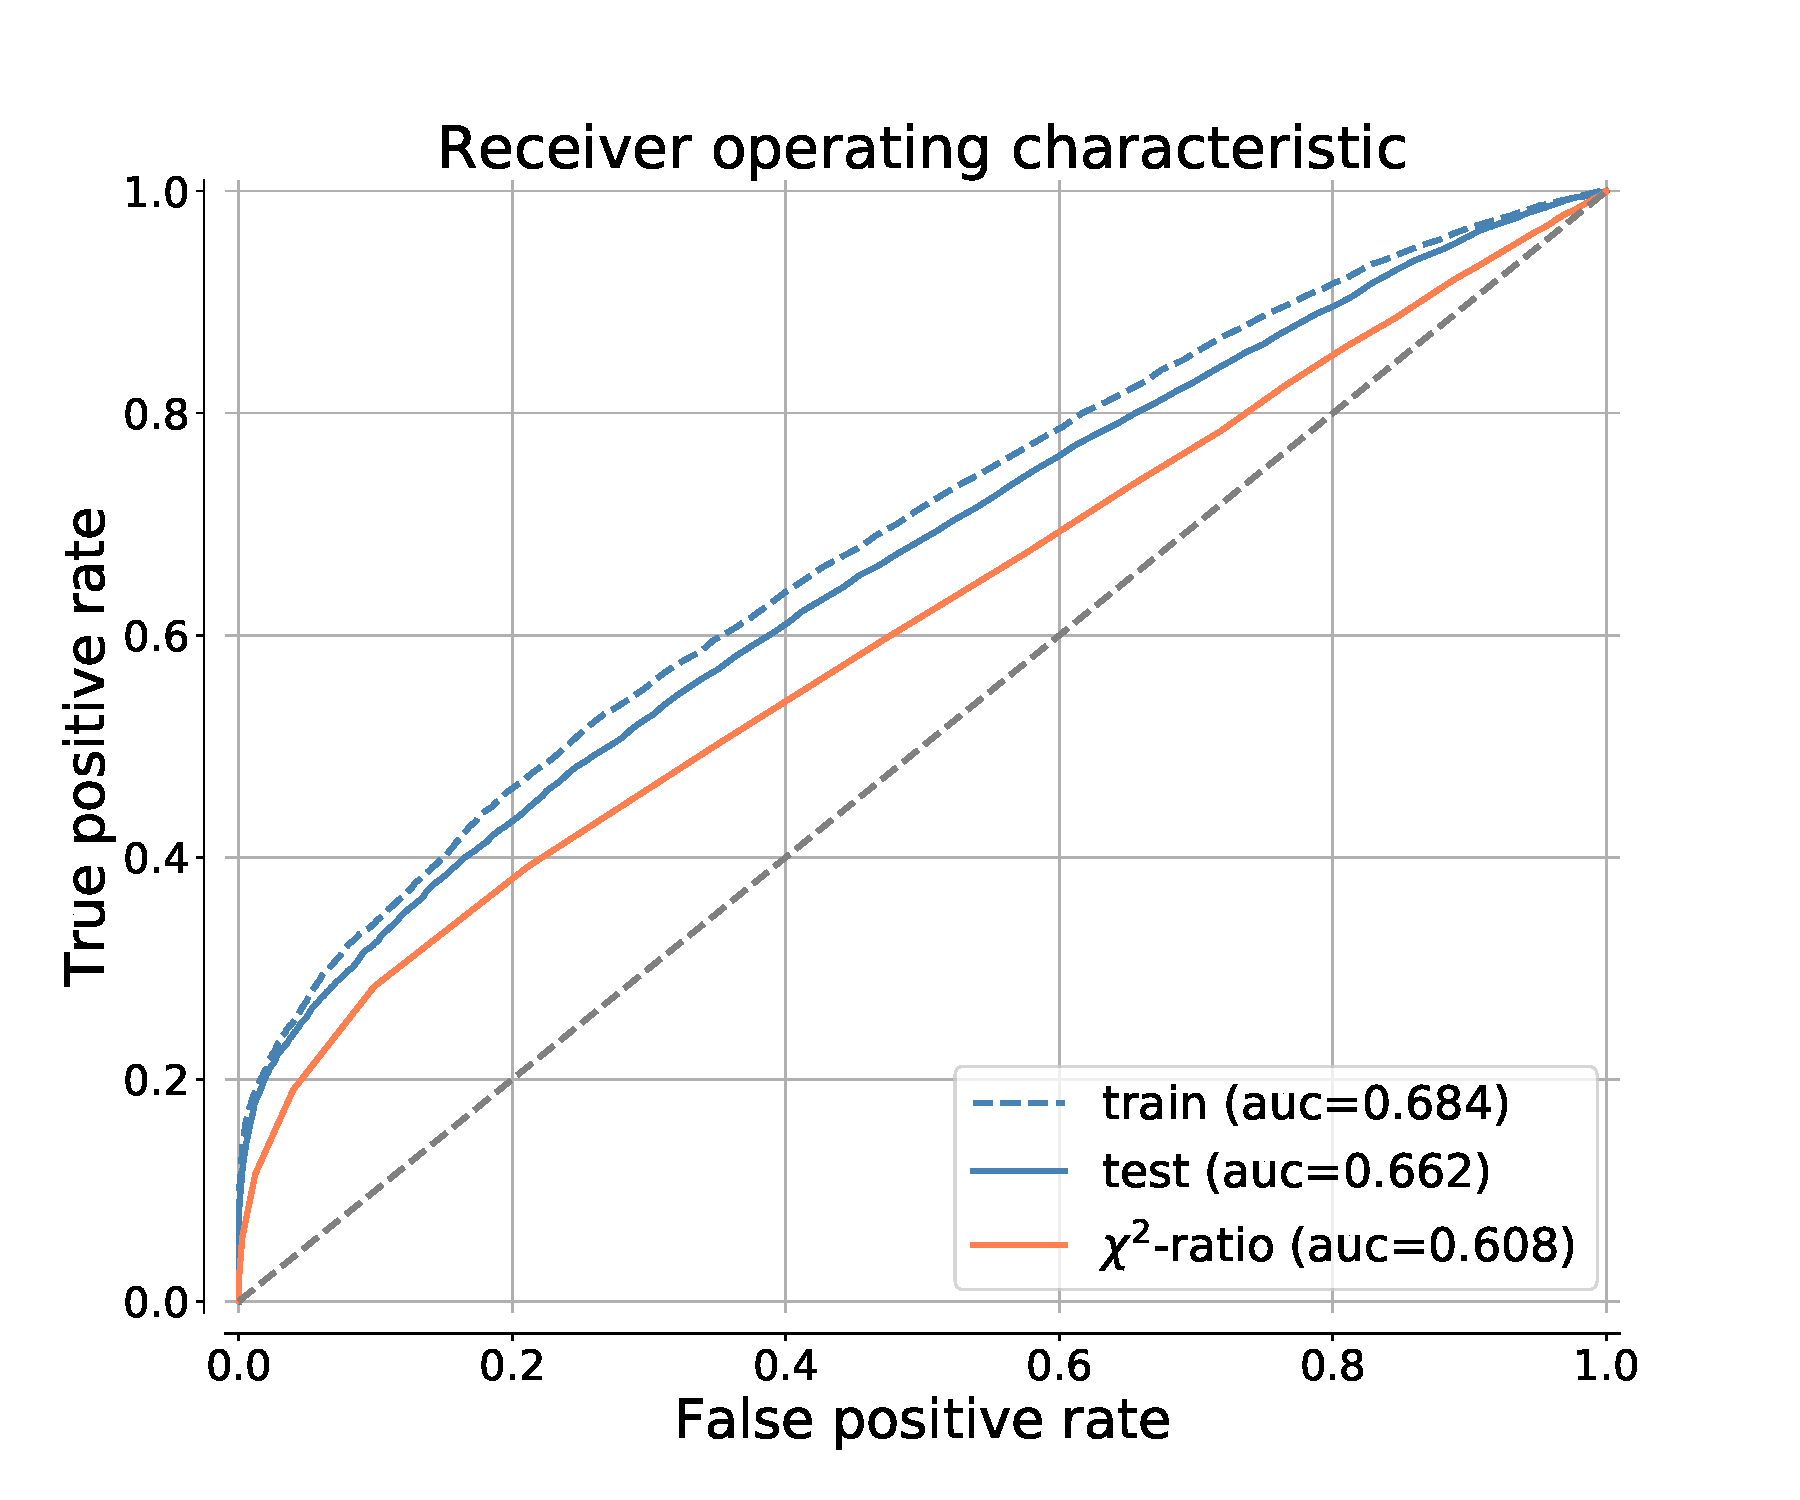
\includegraphics[align=b, trim = 30 25 65 50, clip, width=0.50\linewidth]{figures/roc_curve_compare_only_santa.pdf}
    \label{fig:roc_curve}
    }
    \subfloat[Feature importance]{
    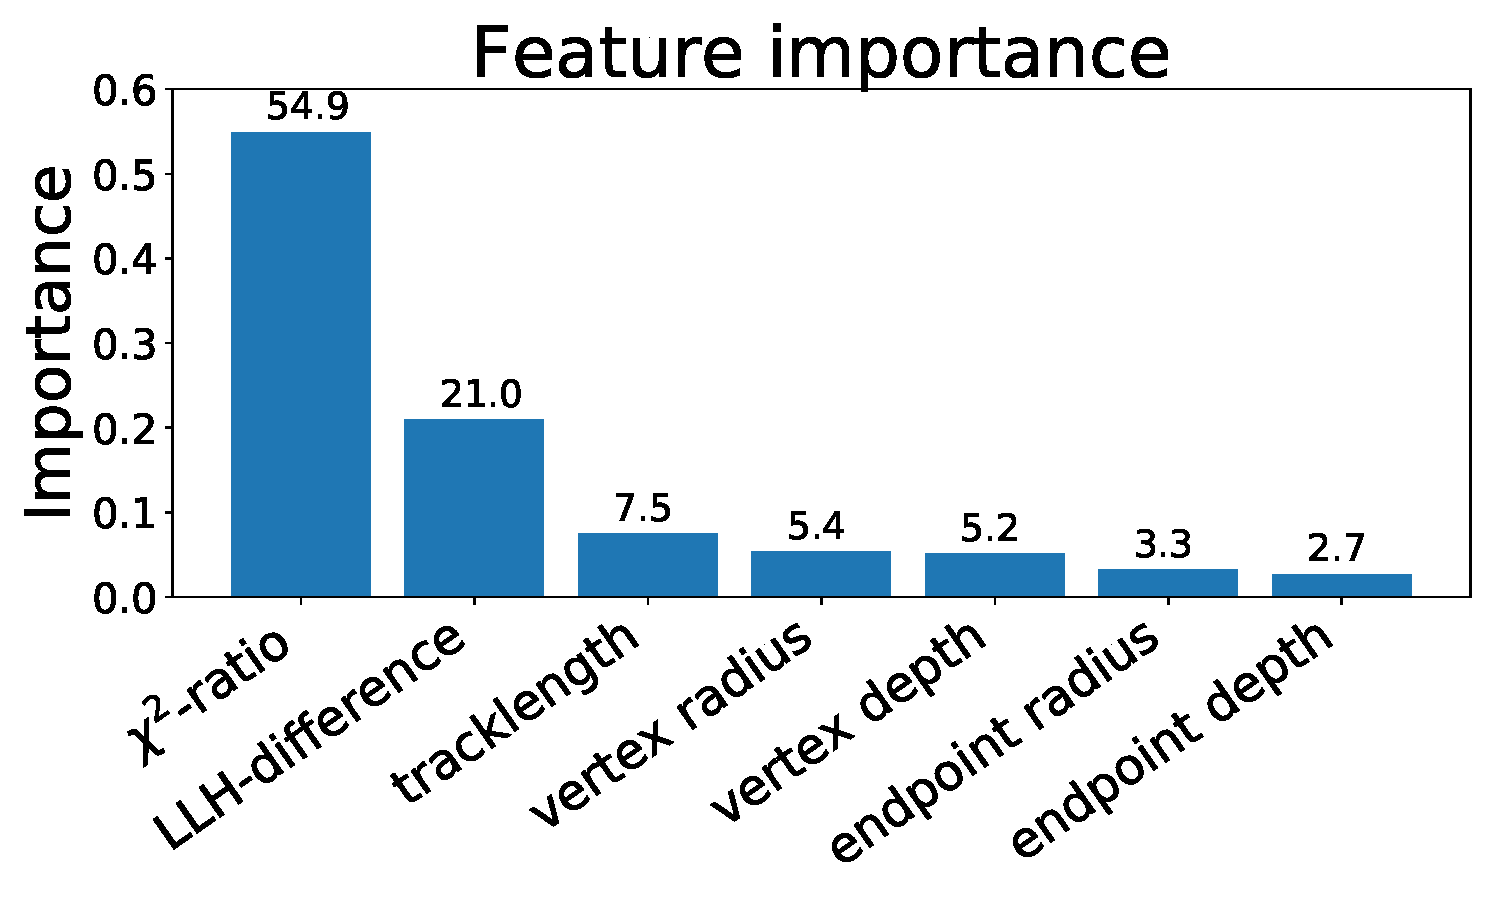
\includegraphics[align=b, width=0.45\linewidth]{figures/feature_importance.pdf}
    \label{fig:feature_importance}
    }
    \caption[Receiver operating characteristic and feature importances for the final, trained classifier]{Receiver operating characteristic and feature importances for final, trained classifier.}
\end{figure}

In Figure~\ref{fig:feature_importance} the relative importances of the various input features are shown.
As already observed from the distributions in Figure~\ref{fig:feature_distributions}, the $\chi^2\textrm{-ratio}$ and the LLH-difference distribution have the strongest effect in separating tracks and cascades with an importance of $55$\,\% and $21$\,\%.
The track length and the spatial coordinates play a lesser role with $3-8$\,\%.
The effect of removing them is tested, but the result is a worse performance of the algorithm, due to the reasons discussed in Section~\ref{sec:feature_selection}.

To illustrate how the trained GBM classifies events coming from the different flavor interactions, the probability score is plotted for the different interactions types individually in Figure~\ref{fig:gbc_probability_flavors}.
On the left, the normalized distribution is shown with a logarithmic y-axis and on the right the cumulative distribution.
\begin{figure}[h]
	\centering
    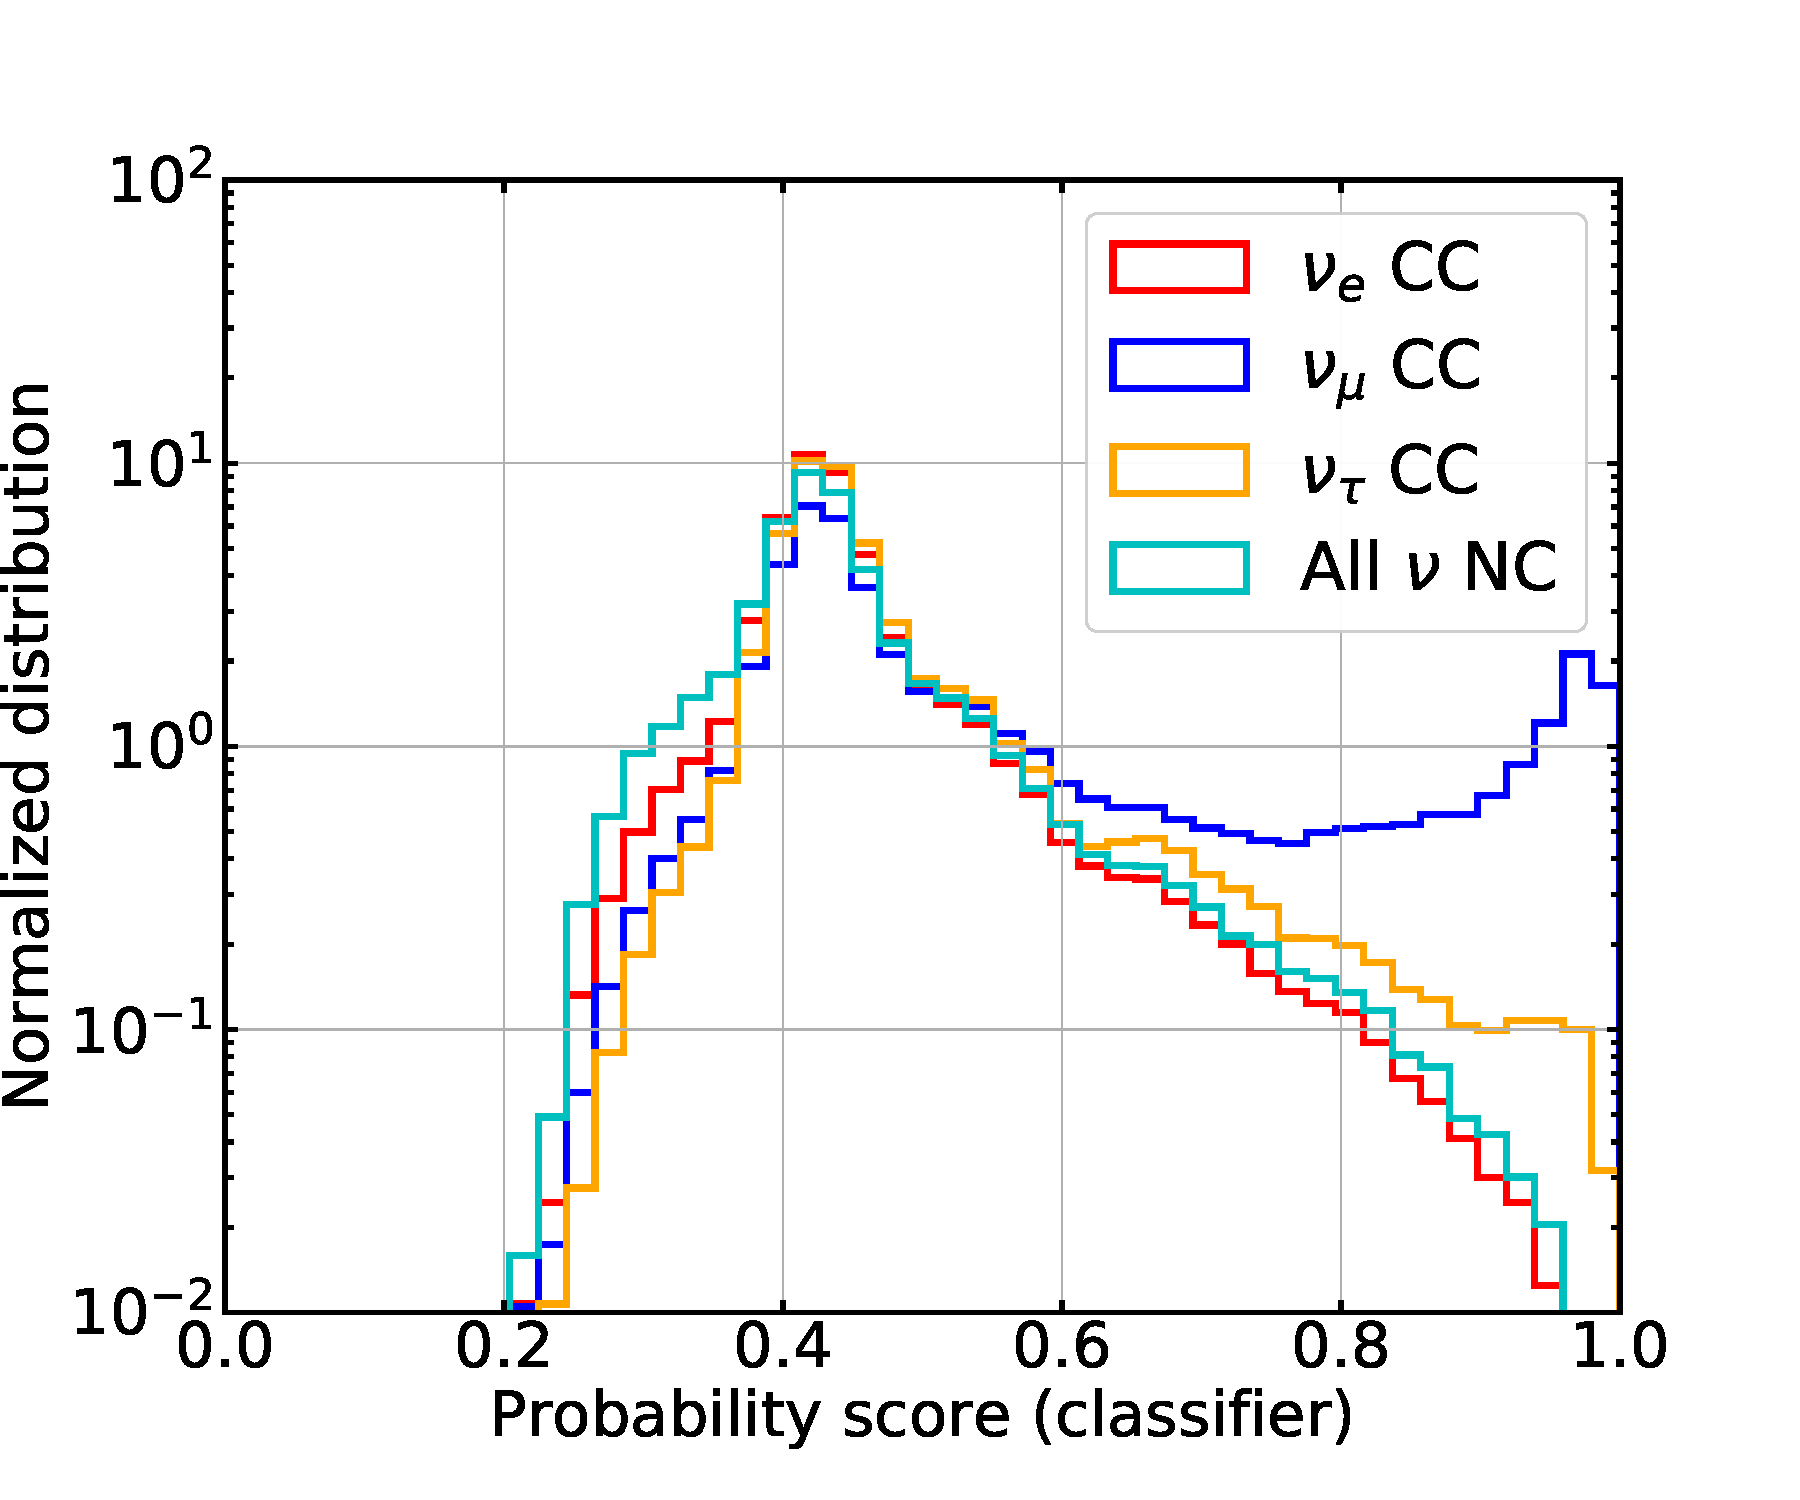
\includegraphics[width=0.49\linewidth]{figures/bdt_score_normalized.pdf}
    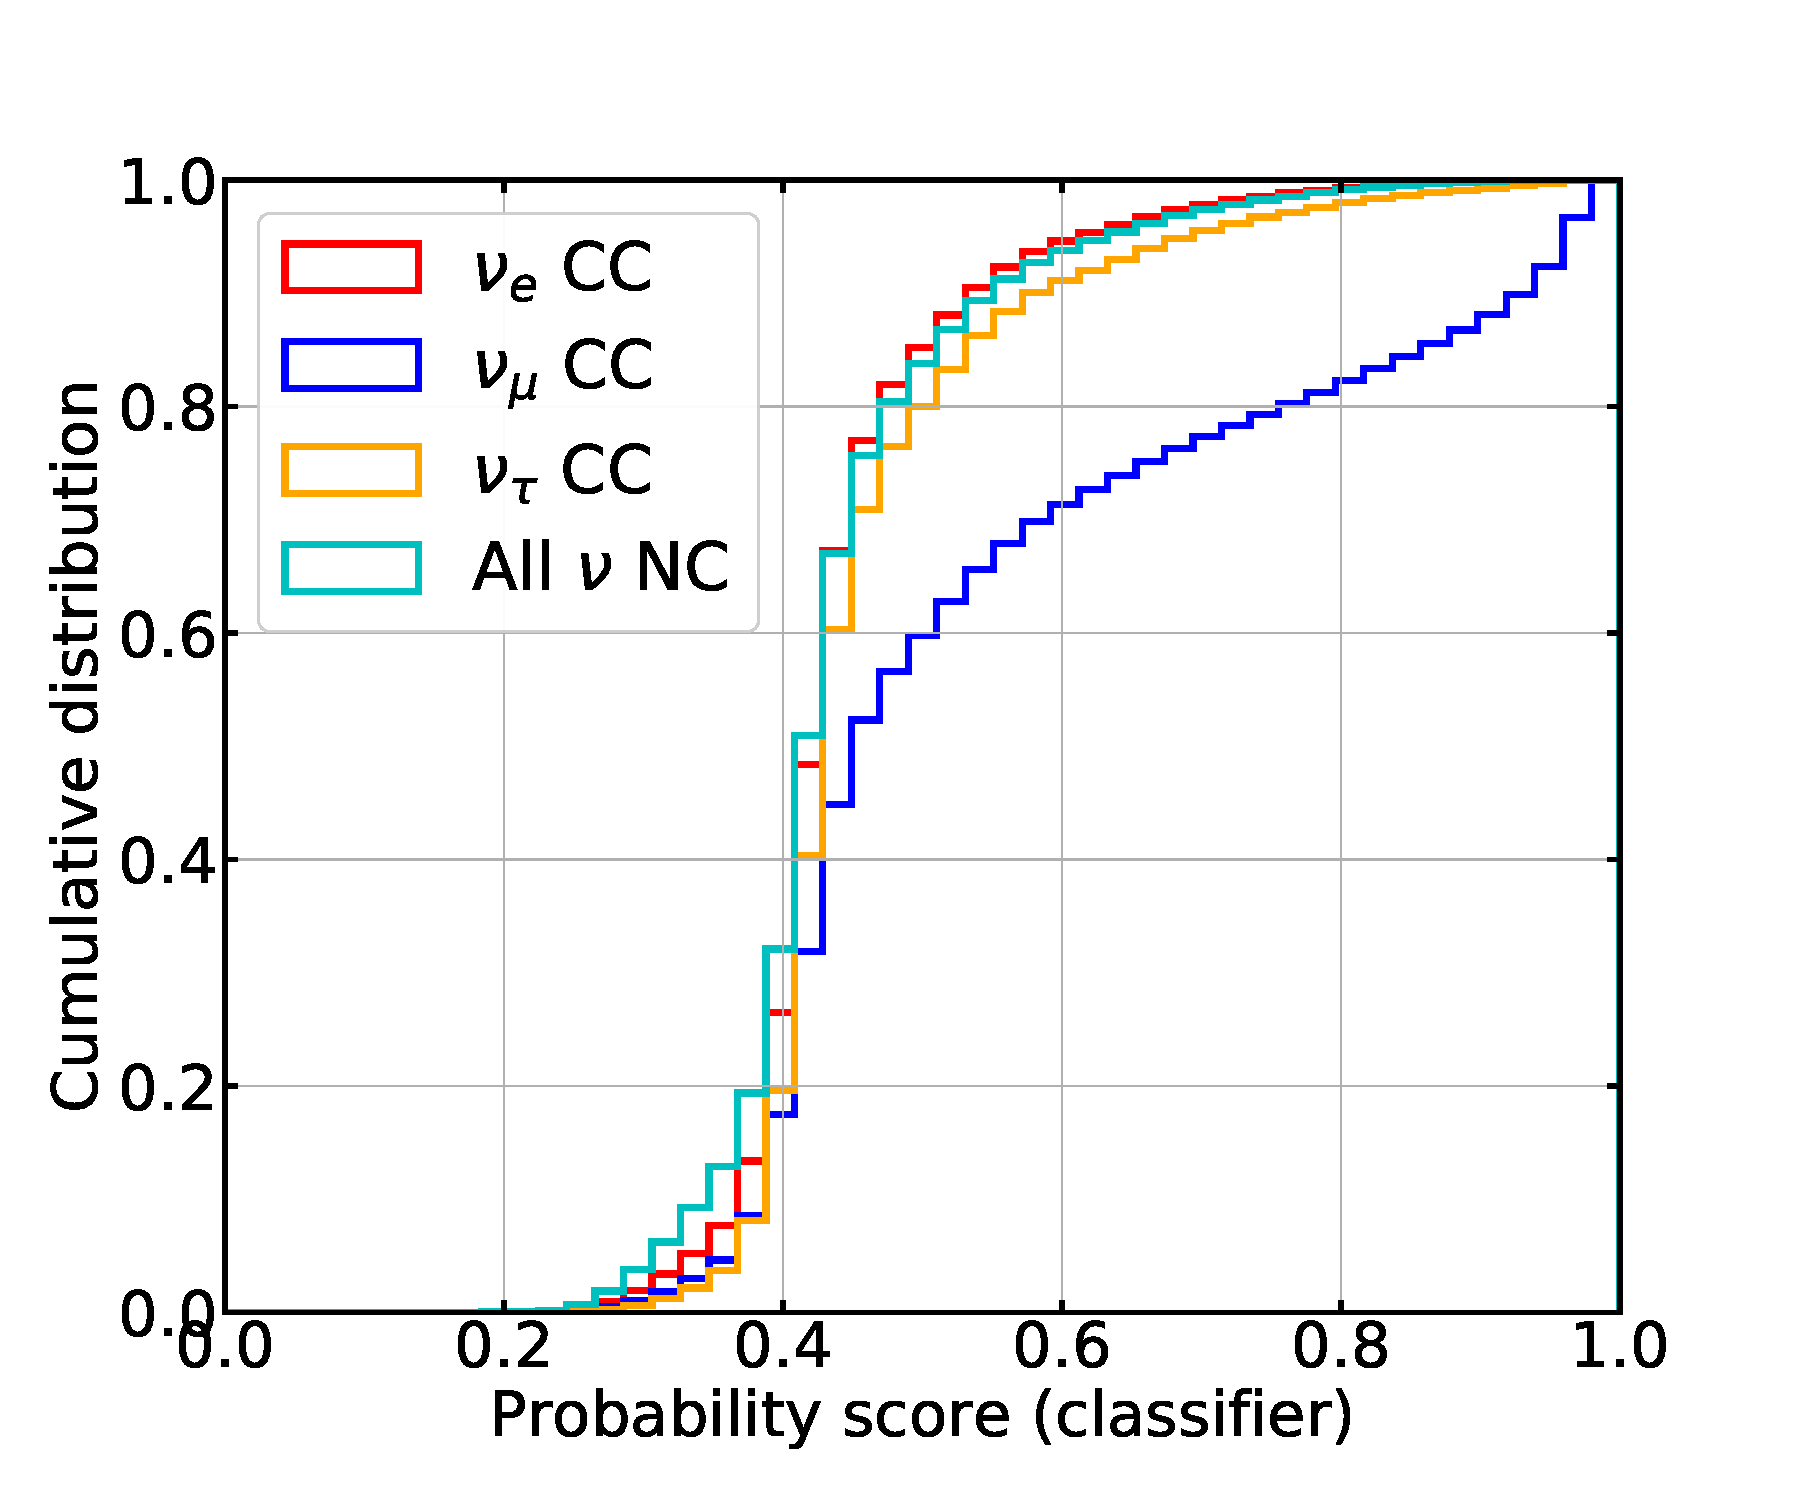
\includegraphics[width=0.49\linewidth]{figures/bdt_score_cumulative.pdf}
    \caption[Expected PID score distribution and the cumulative distribution for the different interaction types]
    {The expected PID score distribution (left) and the cumulative distribution (right) for the different interaction types.}
    \label{fig:gbc_probability_flavors}
\end{figure}
As already discussed before, the $\nu_\mu$-CC event distribution has a clear peak at values of 1 but also spreads towards lower probability values.
It does not have the stronger visible rising edge at probability score values around 0.2-0.3 that the all $\nu$-NC event distributions shows.
This is also weakly observed for the $\nu_e$-CC event distribution. 
The shapes of $\nu_e$-CC event distribution and the all $\nu$-NC event distribution are very similar.
They have their peak at $\sim$0.42 and afterward fall off towards higher probability values.
This behavior makes sense since both $\nu_e$-CC events and the all $\nu$-NC events produce cascade signatures only.
The shape of the $\nu_\tau$-CC event distribution at lower probability values follows the shape of the $\nu_\mu$-CC event distribution.
At higher probability values the $\nu_\tau$-CC event distribution also shows some excess as compared to the $\nu_e$-CC and the all $\nu$-NC event distributions.
This can be explained by the fact that the tau leptons produced in $\nu_\tau$-CC interactions decay to muons with a $17$\,\% BR \cite{PhysRevD.98.030001}.
These events can potentially produce real, visible tracks and the classifier can identify them.

An additional study was performed in oder to test the effect of training the classifier on a sub-set of $\nu_\mu$-CC events.
We trained the classifier on $\nu_\mu$-CC events above a certain threshold track length as true tracks, while adding the remaining fraction of $\nu_\mu$-CC events below the threshold to the cascades.
This approach is motivated by the fact that low energy $\nu_\mu$-CC events have very short tracks and there is a limit below which the detector cannot identify them due to the minimum spatial separation of DOMs.
Although the classifier results achieved with this approach were good, there was no significant improvement in the oscillation parameters sensitivities.
For this reason, the results are not presented here.


\subsection{Classifier Evaluation}

It is necessary to perform certain checks on the trained classifier to guarantee that it performs well.
For example, an algorithm is said to \textit{overfit} when it starts to classify events from known data better than events from unknown data.
Overfitting occurs when the algorithm starts to learn features of the training set that are not general features of the whole dataset, but rather statistical fluctuations.
As a result, the classification of the test set becomes worse.
We can prevent overfitting by comparing the outputs for the training and the test sets.
In Figure~\ref{fig:bdt_probability_distribution} this was done for the distribution of probability scores for true tracks and true cascades separately.
To check whether the distributions match, we calculate the agreement using a two-sided Kolmogorov-Smirnov-test (KS-test) \cite{10010480527}.
The two-sided KS-test checks if the null hypothesis, that two samples are drawn from the same continuous distribution, cannot be rejected.
A high p-value, therefore, means that the two distributions are similar.
For the tracks a p-value of $67$\,\% was found while for the cascades it was $99$\,\%, from which we confirm that there is no overtraining.
In addition to the KS-test, the distributions are compared by their ratio, as shown in the lower part of Figure~\ref{fig:bdt_probability_distribution}.
Apart from the regions where the statistics are low, the ratio is close to 1 and does not show any significant bias.
As it was already done with the input feature distributions, we also check the agreement between data and simulation for the output probability score distribution.
Figure~\ref{fig:bdt_data_mc} shows the comparison plot for the classifier output which shows good agreement between data and simulation.

\begin{figure}[hb]
    \centering
    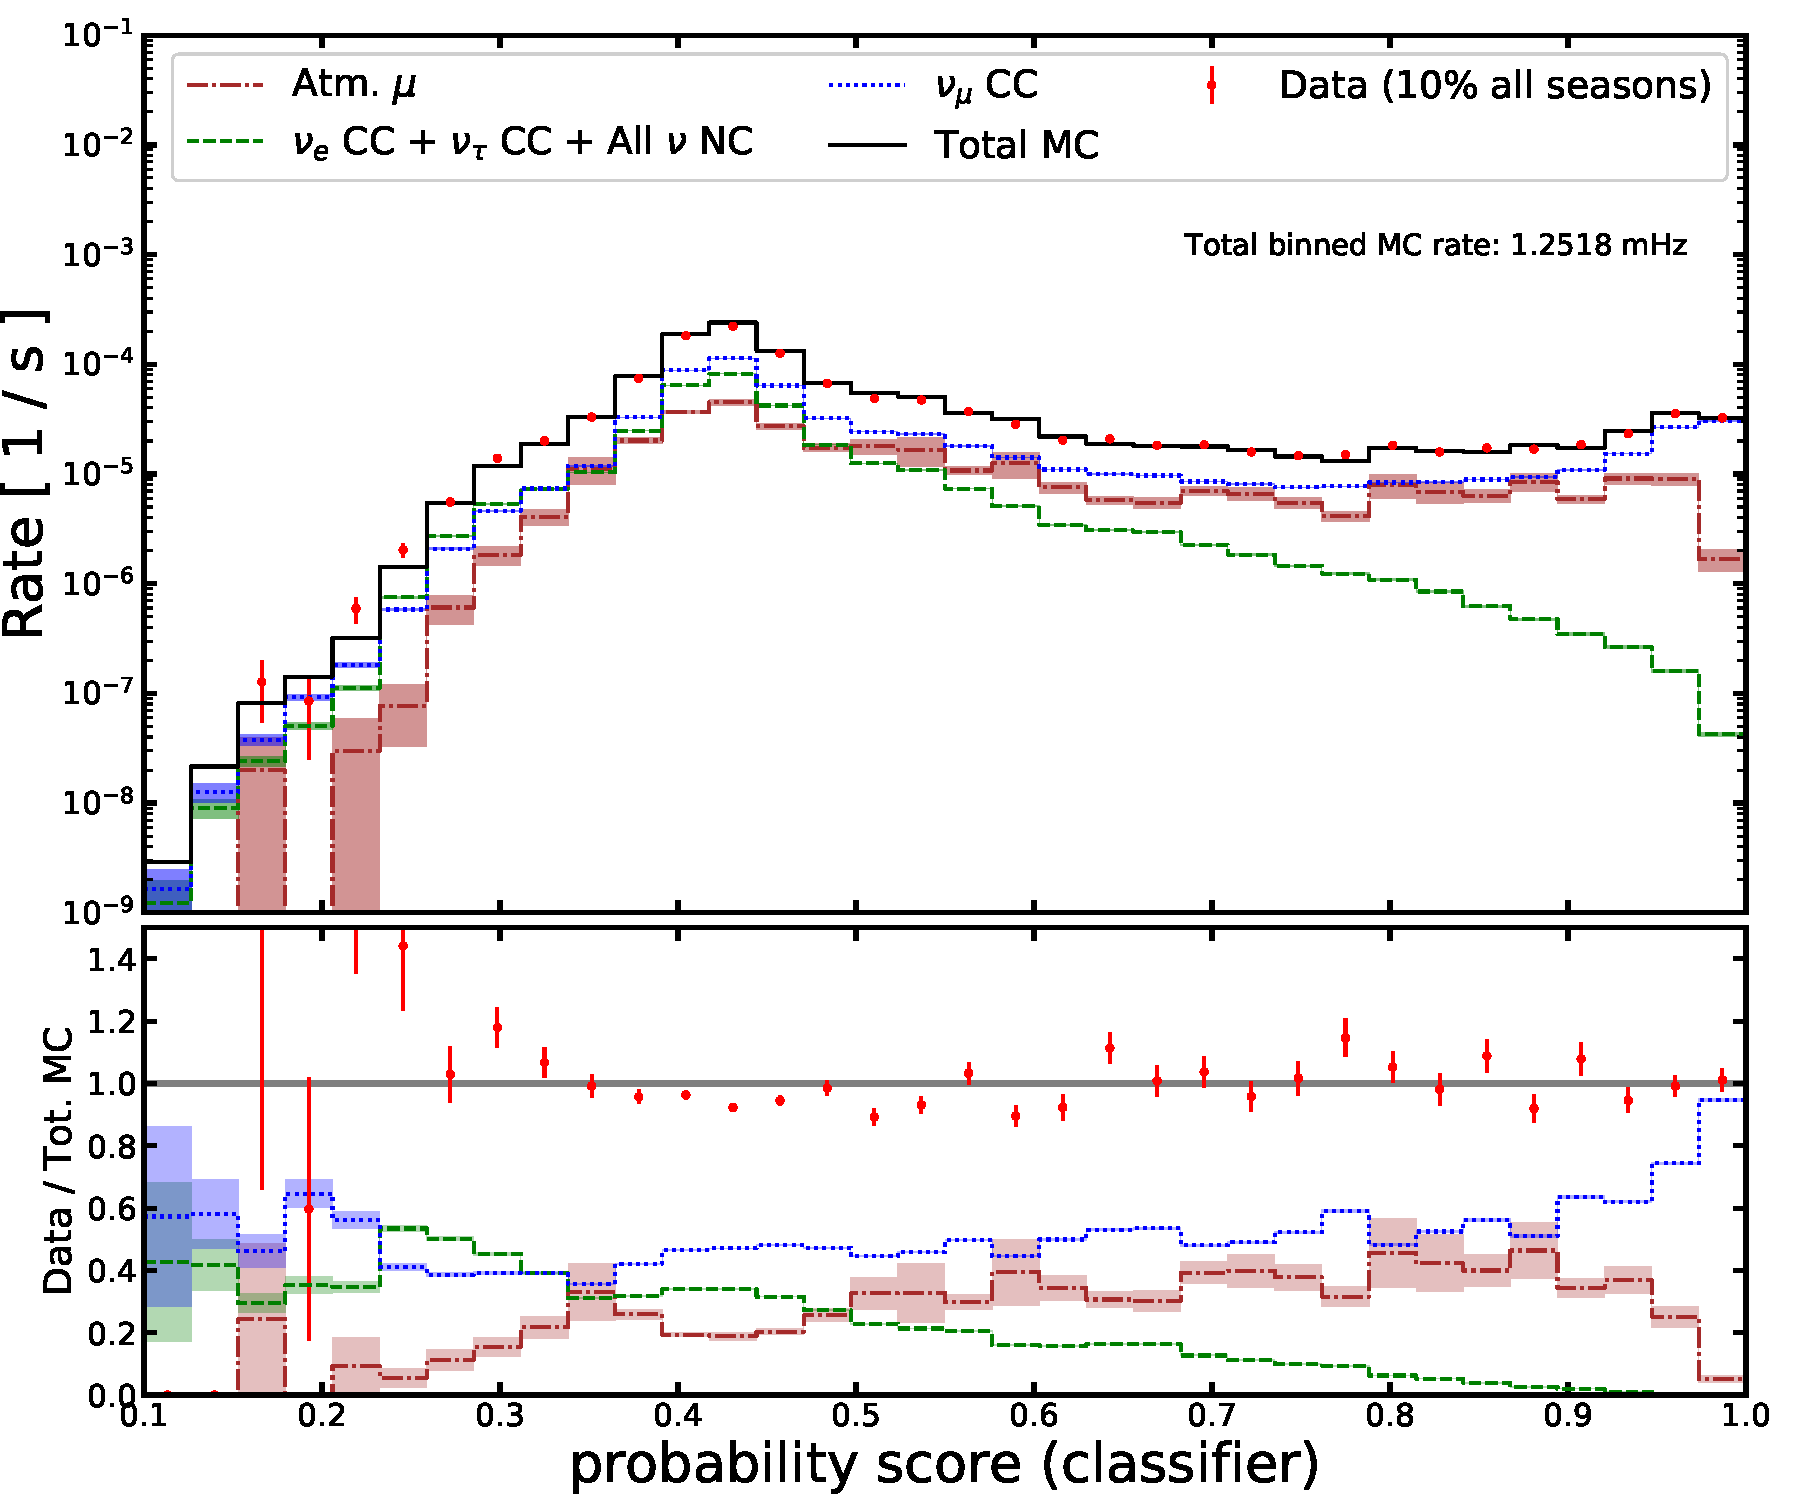
\includegraphics[width=0.9\linewidth]{figures/bdt_score_14.pdf}
    \caption[Data/MC agreement for classifier output probability]{Data/MC agreement for classifier output probability with $\Delta\mathrm{m}^2_{32}=2.42\cdot10^{-3}$\,eV$^2$ and sin$^2\theta_{23}=0.538$.}
    \label{fig:bdt_data_mc}
\end{figure}

Another way to monitor overtraining is related to the ROC curve shown in Figure~\ref{fig:roc_curve}.
For this work, the abilities of the classifier are measured by calculating the area under the curve (AUC) for the ROC curve.
In the ideal case, AUC=1.
A classifier that always classifies the same number of tracks and cascades has a ROC curve following the diagonal between x- and y-axis, which results in an AUC of 0.5.
Such a random classifier has no ability to separate tracks from cascades.
In this work, the AUC is the main metric used to assess the performance of the trained GBM.
Additionally, it provides a method to check for overfitting by comparing the values of the training and test sets.
If we achieve much higher AUC values for the training set than for the test set, it is a clear sign of overfitting.
The AUC values achieved with the trained classifier are $0.684$ and $0.662$ for training and test sets, respectively, and $0.608$ for the $\chi^2$-ratio.
It can be seen that the classifier performs better than the $\chi^2$-ratio and that there exists a region where the TPR is increasing, although the FPR stays close to zero.
This means that for some threshold values, a set of events can be clearly identified as tracks without having any cascade contamination in that chosen track bin.
The AUC score of the training set is not significantly larger than the AUC score of the test set and the classifier, therefore, does not show signs of overfitting.


\subsection{Hyper-Parameter Tuning}

The classifier training process is governed by a set of training variables called hyper-parameters.
Some of them apply to the individual trees while others are related to the boosting algorithm as a whole.
For most datasets, it is useful to modify the parameters of the classifier to achieve the best performance.
In this work we perform a grid-search for every parameter to find the best training output, which is evaluated using AUC as a metric.
The best performing parameters are then used to train the classifier and the usual checks for overtraining and behavior of the classifier are made.
At the start, a set of baseline parameters is chosen to have a comparison when trying to improve the performance.
The tuning of the parameters is essentially done in four steps. In the first step, the learning rate is kept fixed and the best number of estimators is found.
The maximum depth of the trees and the minimum samples required in a node to perform a split are tuned in a second step.
The minimum samples required on a leaf are optimized in a third step to achieve the best training AUC score.
Altering the maximum number of features considered for every split did not improve the score after that, neither did decreasing the learning rate and increasing the number of estimators.

\begin{table}[h]
    \centering
    \begin{tabular} { l || l | l}
        & Default & Tuned \\
        \hline \hline 
        Learning rate & 0.275 & 0.275    \\
        Number of estimators & 50 & 80 \\
        Maximum depth & 3 & 5 \\
        Minimum samples to split & 2 & 1100 \\
        Minimum samples in leaf & 1 & 5 \\
        Maximum features & 7 & 7 \\
        \hline
        AUC(train) & 0.684 & 0.746 \\
        AUC(test) & 0.662 & 0.654
    \end{tabular}
    \caption[Classifier hyper-parameters]{Classifier hyper-parameters before and after the tuning procedure. Also shown is the resulting AUC score for training and test sets.}   
    \label{tab:parameter_tuning}
\end{table}

The default parameters, as well as the tuned parameters are shown in Table~\ref{tab:parameter_tuning}.
Also shown is the overall score on training and test sets after the classifier training with the new parameters.
Evidently, tuning the hyper-parameters did increase the AUC score on the training set, but for the test set, it led to degradation.
This is a clear sign of overtraining since the tuning solely affects the performance on the training set.
We also see large discrepancies when checking the probability score distributions for training and test sets shown in Figure~\ref{fig:probability_distribution_tuned}.
The probability distributions for the training and test sets using the tuned parameter set do not agree with each other.
This is particularly the case for the cascade distributions.

This exercise demonstrates the trade-off between hyper-parameter tuning and overtraining.
It also shows that to perform a proper hyper-parameter tuning the simulation statistics are not sufficient.
Therefore, we use the default parameters listed in Table~\ref{tab:parameter_tuning} since they do not result in overtraining.

\begin{figure}[h!]
    \centering
    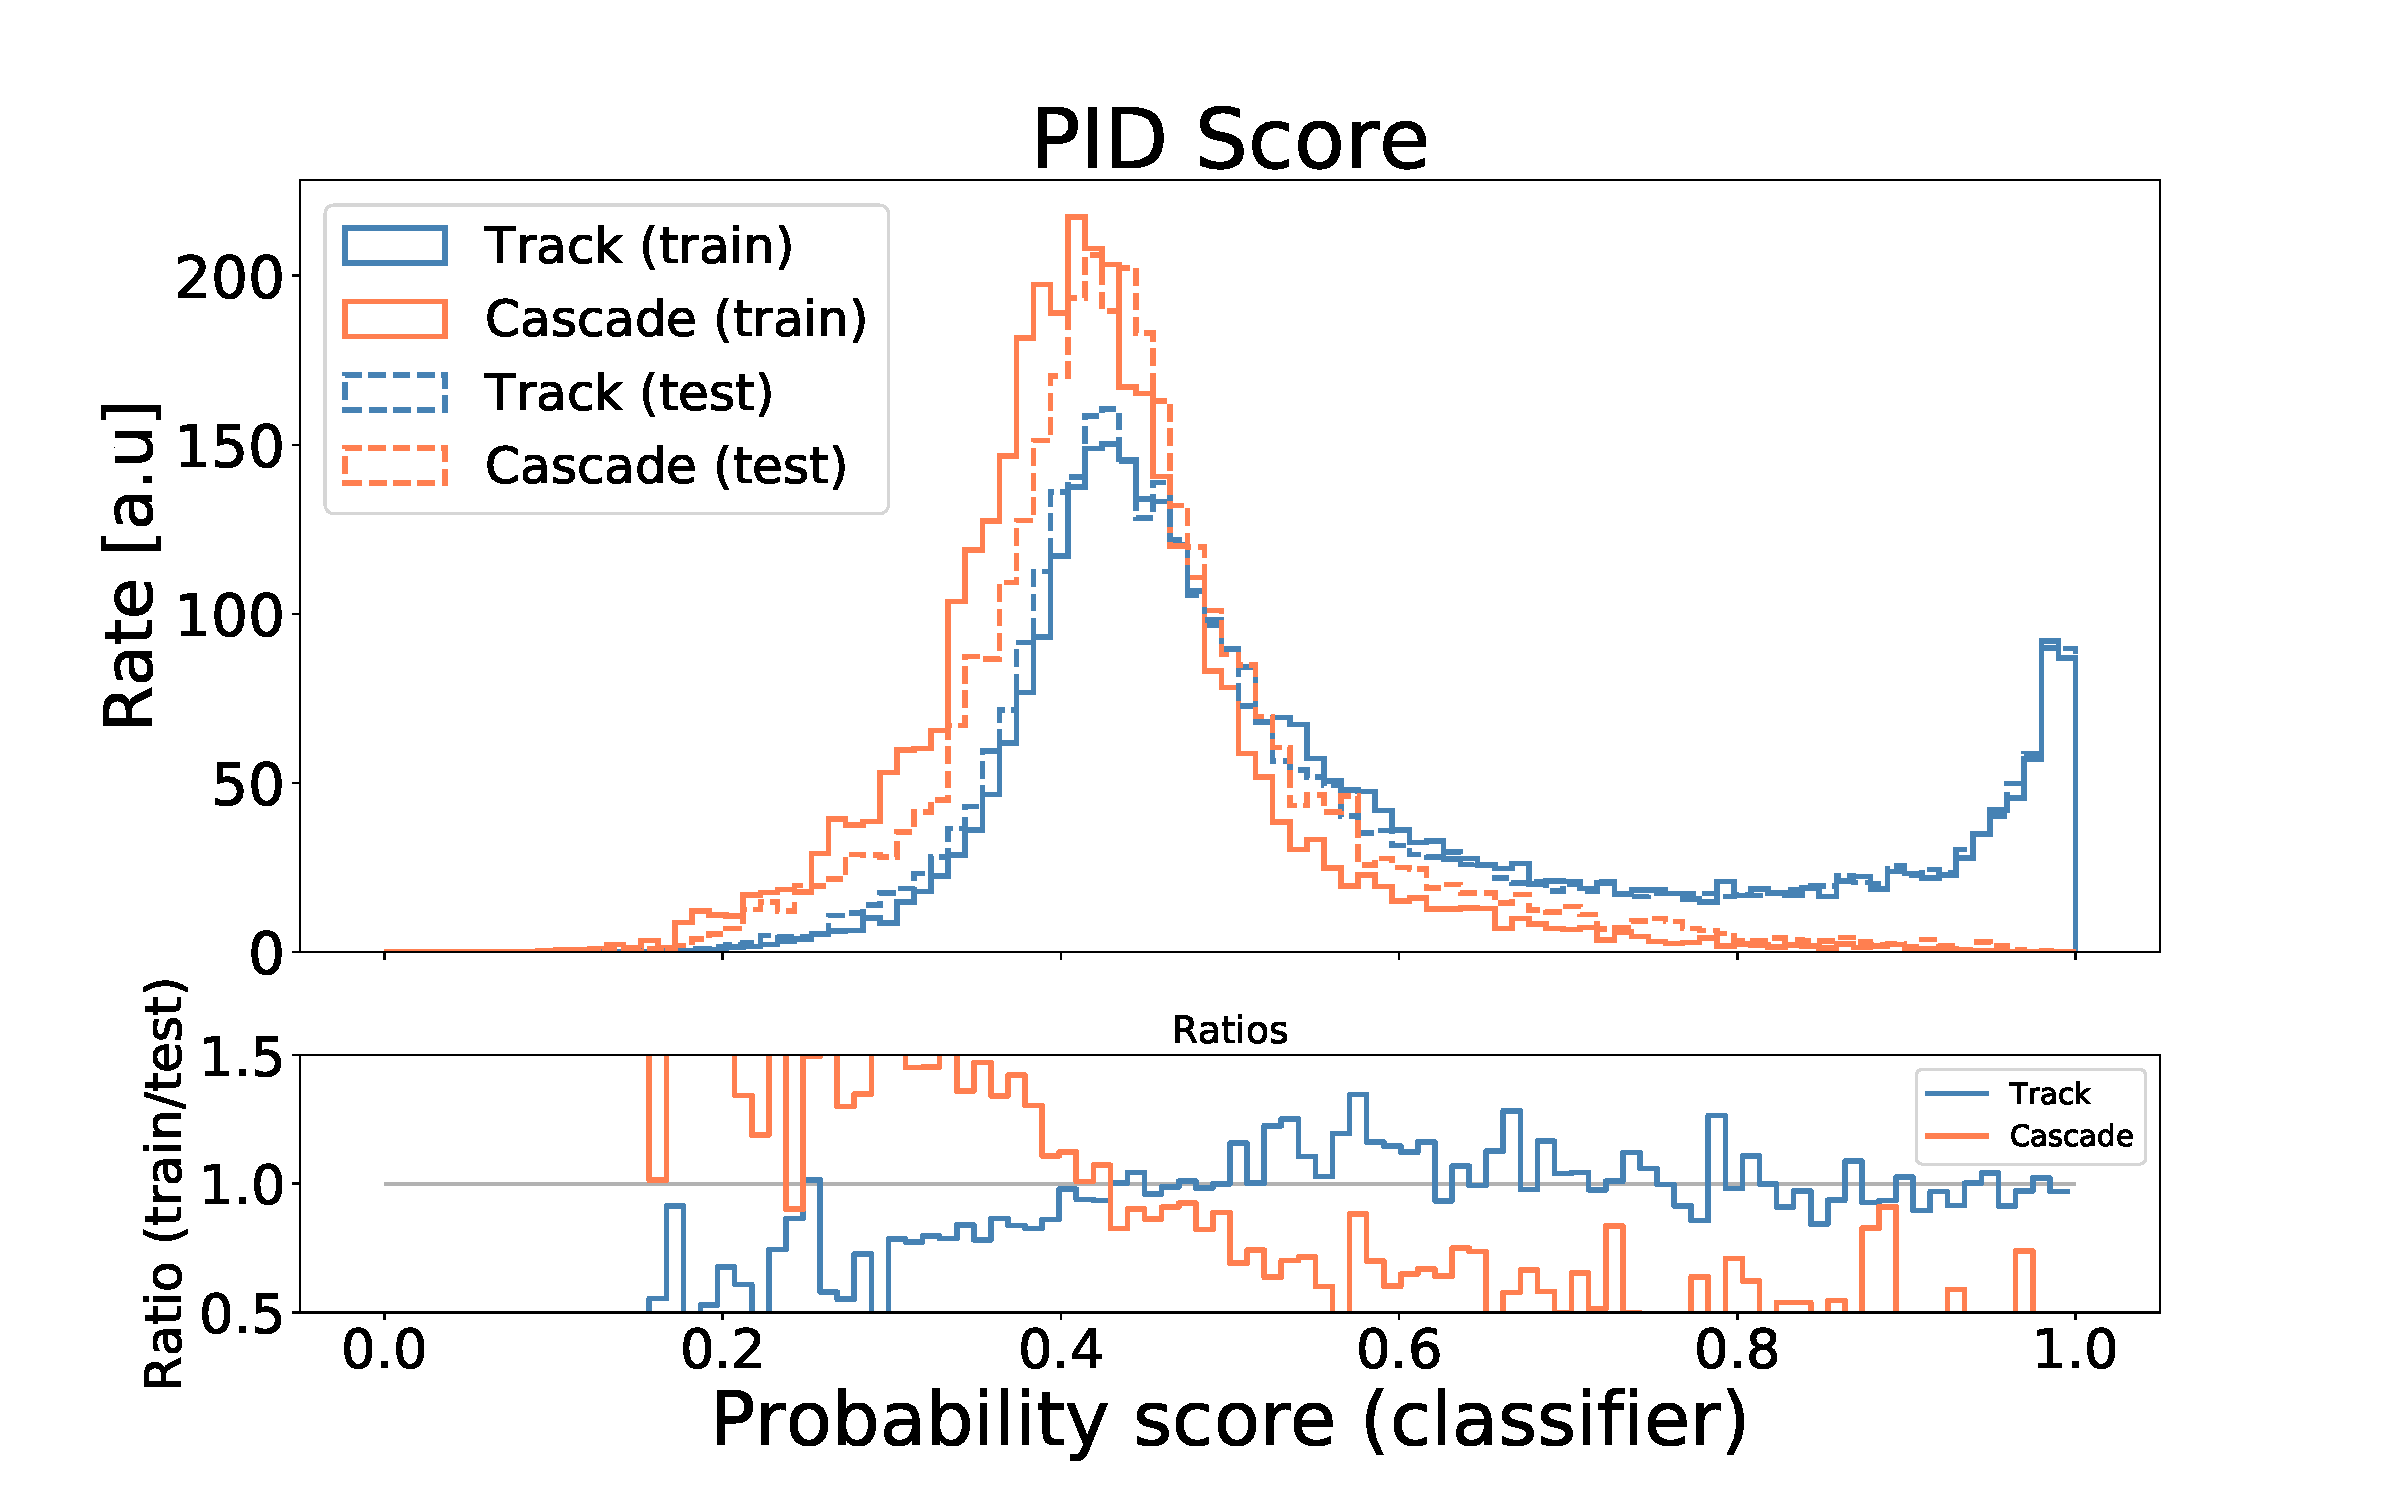
\includegraphics[trim = 35 05 110 25, clip, width=0.8\linewidth]{figures/probability_distribution_step5_neu.pdf}
    \caption[Classifier output probability with tuned parameters]{Classifier output probability with tuned parameters for training/test set split in $\nu_\mu$-CC (track) and $\nu_e$-CC+$\nu_e$-NC+$\nu_\mu$-NC (cascade).}
    \label{fig:probability_distribution_tuned}
\end{figure}
